%%%%%%%%%%%%%%%%%%%%%%%%%%%%%%%%%%%%%%%%%%%%%%%%%%%%%%%%%%%
% EPFL report package, main thesis file
% Goal: provide formatting for theses and project reports
% Author: Mathias Payer <mathias.payer@epfl.ch>
%
% This work may be distributed and/or modified under the
% conditions of the LaTeX Project Public License, either version 1.3
% of this license or (at your option) any later version.
% The latest version of this license is in
%   http://www.latex-project.org/lppl.txt
%
%%%%%%%%%%%%%%%%%%%%%%%%%%%%%%%%%%%%%%%%%%%%%%%%%%%%%%%%%%%
\documentclass[a4paper,11pt,oneside]{report}
% Options: MScThesis, BScThesis, MScProject, BScProject
\usepackage[MScThesis,lablogo]{EPFLreport}
\usepackage{datetime}
\usepackage{amsmath}
\usepackage{amssymb}
\usepackage{xspace}
\usepackage{array}
\usepackage{lscape}
\usepackage{booktabs}
\usepackage{subcaption}
\usepackage{gensymb}
\usepackage{stmaryrd}
\usepackage{verbatim}
\usepackage{siunitx}
\usepackage{algpseudocode}
\usepackage{algorithm}
\usepackage{parskip}



\usepackage{hyperref}
\usepackage{graphicx}


\title{Regional Surface Mass Balance Emulator based on Deep Learning: \\ local-scale SMB predictions over the Antarctic Peninsula}
\author{Marijn van der Meer}
\supervisor{Sophie de Roda Husman}
\adviser{Prof. Dr. sc. EPFL Martin Jäggi}
\expert{Prof. Dr. sc. TU Delft Stef Lhermitte}

\newcommand{\sysname}{FooSystem\xspace}

\begin{document}
\maketitle
\dedication{
\begin{raggedleft}
    Nevertheless, she persisted.\\
    --- \\
\end{raggedleft}
\vspace{4cm}
\begin{center}
    
Diese Arbeit ist meiner Grossmutter Brigitte Dorigo Baumann gewidmet. Danke liebes Grosi, für all deine Unterstüzung, ich habe dich sehr lieb.\\
-- \\
Thank you also to my parents, Jan Roelof van der Meer and Barbara Baumann, who have always been my biggest inspiration to join the scientific world through their work and dedication. 
\end{center}}

\makededication

\acknowledgments{I would like to express my deep gratitude to Prof. Stef Lhermitte and Prof. Martin Jäggi, my thesis supervisors, for their patient guidance, enthusiastic encouragement, and valuable critiques of this research work. I would also like to thank Sophie de Roda Husman for her helpful advice and assistance on my thesis.

I would like to express my special thanks to Christoph Kittel for providing me with the MAR(ACCESS1.3) RCM dataset and for his availability to answer my questions. Likewise, I would like to thank Doury et al.'s team for providing me with information about their RCM-emulator. 

I would like to thank my proofreaders in order of occurrence but not of importance: Melissa Corboz, Jan Roelof van der Meer, Jantina van der Meer, and Maxime Fellrath. 

Last but not least, I would like to thank my dear friends and family, whose love and support kept me motivated and confident.


Finally, I would like to thank Prof. Payer from the EPFL for creating the practical latex package to write this EPFL thesis. The latest version of this package is available \href{https://github.com/HexHive/thesis_template}{here}.}

\makeacks

\begin{abstract}
Surface mass balance (SMB), a measure of processes leading to the addition or removal of ice, is crucial in controlling the stability and dynamics of the Antarctic ice sheet. It is imperative to have precise estimations of the local SMB to predict Antarctic ice sheet variations and sea-level rise. Currently, however, it is challenging to model SMB correctly because of its high variability across space and time and its complex interactivity with atmospheric variables. In this thesis, we developed a machine learning framework that learns to create local SMB predictions from global-scale climate model (GCM) outputs, which are readily available. We focused on the Antarctic Peninsula, the fastest warming region of the Antarctic ice sheet, which loses ice mass at significant rates. For this, detailed SMB predictions were available from the MAR(ACCESS1.3) regional climate model dataset (RCM). We built the RCM-emulator using a U-Net with convolutional block attention mechanisms, depth-wise separable convolutions, and a normalized RMSE loss. To train the emulator, we proposed two frameworks. In the first, called the perfect model framework, the RCM-emulator received upscaled RCM features at GCM resolution ($\mathrm{\hat{F}_{U}}$) instead of low-resolution inputs from the GCM. In this case, the model learns only the RCM downscaling function and is undisturbed by potential RCM-GCM inconsistencies and biases. $\mathrm{\hat{F}_{U}}$ was evaluated both on upscaled RCM and GCM features. In the second framework, we trained the emulator with large-scale features directly sourced from the GCM ($\mathrm{\hat{F}_{G}}$) to evaluate whether it could make accurate predictions despite RCM-GCM inconsistencies. Our results show that $\mathrm{\hat{F}_{U}}$ can almost perfectly reproduce the high-resolution SMB truth from upscaled RCM features. However, its predictions from GCM features lead to consistent underestimation of true SMB. In contrast, $\mathrm{\hat{F}_{G}}$ can reproduce the true SMB values successfully from GCM, and despite large-scale bias between the GCM and RCM, except for very dry regions. This suggests that the RCM-emulator can work directly with GCM data rather than with a perfect model framework because it can learn the proper GCM to RCM downscaling. The emulator also presents a large computational gain compared to running an RCM simulation, with training under ten minutes and predictions in a few seconds. 

We conclude that machine learning emulators can be applied to produce fast and fine-scaled reproductions of RCM simulations from GCM data. Therefore, they can be an interesting tool for providing low-cost local-scale information on the ice sheet evolution and dynamics in a changing climate. 




    

\end{abstract}

\begin{plainlanguage}

The Antarctic ice sheet contains the majority of ice on Earth and would be the most significant contributor to sea-level rise if it were to melt completely. A critical variable in studying the stability and evolution of ice on Antarctica, such as glaciers and ice shelves, is surface mass balance (SMB). SMB is the balance between processes that add and remove ice on top of an ice sheet, glacier, or ice shelf. For example, those processes can include snowfall, surface melt, or erosion by winds. To predict changes in the Antarctic ice sheet, climate scientists need highly detailed information about SMB. 

High-resolution maps of SMB are usually only produced by regional climate models (RCM). But these are costly and time-consuming to create because they require calculations on very powerful computers. The goal of this project was to accomplish this faster and with similar accuracy by using machine learning to predict SMB changes. 

We trained a machine-learning algorithm i.e., a computer program that recognizes patterns in data, to learn the relationship between a group of low-resolution images of climate variables and a high-resolution image of regional SMB. The low-resolution data consisted of a bundle of atmospheric variables influencing SMB, such as precipitation, temperature, and surface pressure over the Antarctic Peninsula, an interesting region of Antarctica. Those coarse-grain atmospheric variables are easier and cheaper to obtain from worldwide simulations made by climate scientists. 

Our machine-learning model can recreate regional images of SMB almost identical to ground truth observations by learning the relationship between low and high-resolution inputs. The model only struggles to predict proper SMB values for very dry areas (where the SMB is small) because it tends to emphasize points with larger changes in SMB. The predictive model is very fast, with training under ten minutes and output in a few seconds. What remains to be studied is whether the model would need new training for every new (unseen) region in Antarctica or if it could be deployed across areas.

We conclude that it is possible to make fast and detailed reproductions of SMB at regional scales using machine learning. Therefore, machine learning can be an interesting and cheap tool for gathering local-scale information about how ice sheets vary with climate change.  


\end{plainlanguage}

\begin{comment}
\begin{frenchabstract}
For a doctoral thesis, you have to provide a French translation of the
English abstract. For other projects this is optional.
\end{frenchabstract}
\end{comment}

\maketoc

%%%%%%%%%%%%%%%%%%%%%%
\chapter{Introduction}
%%%%%%%%%%%%%%%%%%%%%%


%\textbf{Paragraph 1}-\textit{Discuss the setting, Antarctic ice sheet and SMB. Why is SMB important? Climate change, stability of AIS, sea-level rise, etc.}
    
    The Antarctic ice sheet\footnote{Ice sheet, otherwise referred to as a continental glacier, is a mass of glacial ice that covers land and is greater than 50'000 \si{km^2}. The only present-day ice sheets are in Antarctica and Greenland~\cite{Icesheet}.} (AIS) is the largest class of glaciers and contains the majority of ice on Earth, with a volume of 30 million cubic kilometers~\cite{Icesheetsquick}. It extends over 14 million square kilometers, roughly the combined areas of the US and Mexico~\cite{AntarcticIceSheet}. This amount of ice constantly changes through melting processes and the addition of new mass from snow and ice. 
    
    Since the early 1900s, numerous glaciers worldwide have been melting at high rates due to human activity~\cite{WWF}. 
    If the AIS were to melt entirely, sea-levels would rise by approximately 60 \si{m}~\cite{Kittel, Fretwell, Morlighem}, making the AIS the most significant potential contributor to sea-level rise. Indeed, the AIS has been steadily losing ice mass since 2002~\cite{Shepherd, Mottram}, mainly because of calving\footnote{Calving is the process of chunks of ice breaking off from the edge of a glacier~\cite{Marshak}.} and melting at the water-ice interface underneath ice shelves\footnote{Ice shelves are floating ice that is connected to a continental landmass~\cite{iceshelvescollapse}.} (basal melting)~\cite{Kittel, Mottram, Rignot}. In the case of grounded ice, this water flows into the oceans and directly affects sea-level rise~\cite{icesheet}. Antarctic ice can also indirectly contribute to sea-level rise through, for example, the collapse of ice shelves. Ice shelves are floating ice formed by the extension of grounded ice at the coastline, and they restrict the direct flow of the glaciers into the ocean. Because they float on the water, they do not contribute directly to sea-level rise, but if they break, the ice flow of grounded ice into the water can speed up and lead to sea-level rise~\cite{Hartley2020, iceshelvescollapse}.  
    
    
    A primary variable used to observe the AIS is surface mass balance (SMB). SMB is the net balance between inputs and outputs of mass i.e., ice, snow, and water, on top of the ice sheet (\autoref{fig:example-smb-and-processes})~\cite{Lenaerts2019}. It is influenced by the addition of mass through precipitation and snow‐transporting winds and ablation via wind erosion and sublimation~\cite{Kittel}. At any point, SMB close to zero indicates an arid climate with little change in the ice mass, while a positive SMB means that mass was added, through precipitation, for example. Inversely, a negative SMB indicates that a glacier is losing mass on the surface. SMB is highly important in monitoring the ice sheet's stability and evolution. Changes in surface mass of the AIS impact the global mass balance\footnote{Mass balance is the balance of overall mass, not only at the surface, gained by snow deposition, and the loss of mass by melting and calving~\cite{icesheet}.} and therefore, the ice dynamics and sea-level rise~\cite{Mottram}. Thus, it is imperative to correctly estimate the SMB of the AIS~\cite{icesheet}. Currently, however, it is challenging to model SMB accurately.  

    
    %% SMB figure:
    \begin{figure}[tbp]
        \centering
        \begin{subfigure}[b]{0.45\columnwidth}  
            \centering 
            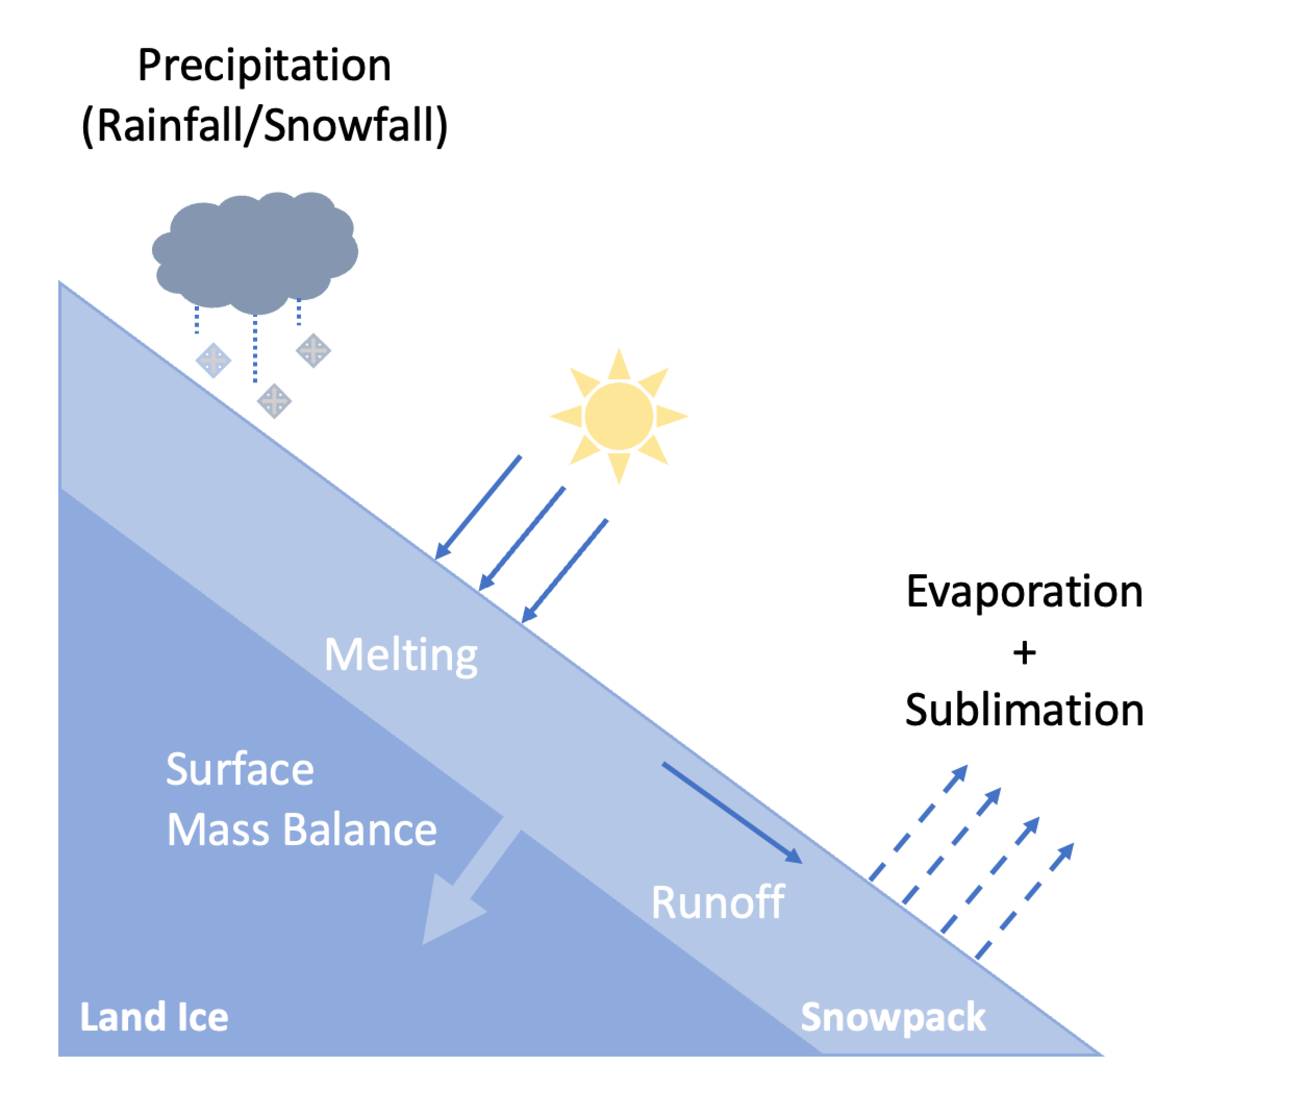
\includegraphics[width=\textwidth]{doc/Thesis-latex/images/processes_smb.pdf}
            \caption[]%
            {{\small }} \label{fig:smb-processes}
        \end{subfigure}
        \hfill
        \begin{subfigure}[b]{0.45\columnwidth}
            \centering 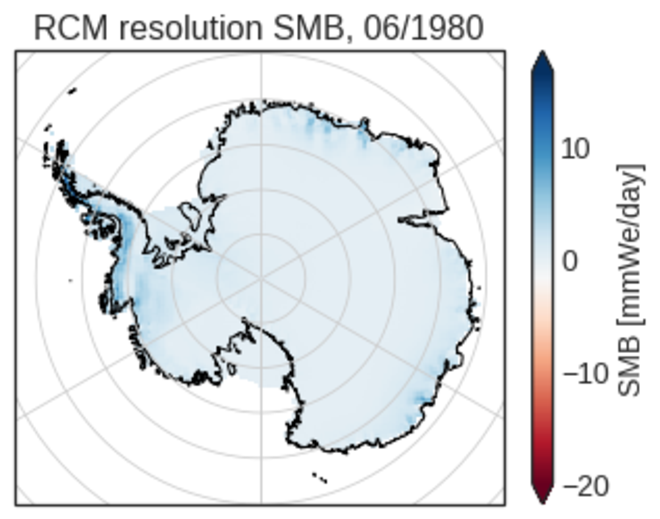
\includegraphics[width=\textwidth]{doc/Thesis-latex/images/smb-example.pdf}
            \caption[]%
            {{\small }}    
          \label{fig:example-smb}
        \end{subfigure}
        \caption[]
        {\small (a): Illustration of processes influencing the surface mass balance (SMB) on the Antarctic ice sheet. (b) Example of daily SMB values aggregated over a random month (06/1980) over Antarctica at regional climate model resolution.
        } 
        \label{fig:example-smb-and-processes}
    \end{figure}
    
% \textbf{Paragraph 2} - \textit{Introduce the main challenges that we see: modeling SMB is very difficult. Done mainly with climate simulations but computationally expensive.}
    
Although SMB can be monitored with on-site tools (e.g., geodetic mass balance stakes), the vastness and climate of Antarctica make these expeditions challenging~\cite{Lenaerts2019}. A more reasonable alternative is to extrapolate SMB in high-resolution\footnote{Note here that by low-resolution, we mean large-scale coarse images (e.g. 50-300 \si{km}); by high resolution, we mean local-scale fine images (e.g. 1-50 \si{km}).} climate model predictions~\cite{Mottram}. To understand and predict the behavior of different climate phenomena, climatologists have developed complex climate models, which are simulations of climate variables over time and space in different parts of the world. However, at our current technological level, the complexity of these climate models is a compromise between computational costs, resolution of pixels, and the domain covered~\cite{Doury}. Depending on the spatial resolution, two types of climate models are typically defined: global (GCM) and regional (RCM). GCMs are simulations that cover the whole planet. They are relatively cheap in terms of computational costs because their domain size (i.e., the geographical region covered) is wide, while their spatial resolution is low (50-300 \si{km})~\cite{Doury}. Unfortunately, for a fine-scale representation of the AIS, such as its edges or peripheral ice, the resolution of a GCM is too coarse~\cite{Kittel, Seroussi}. In addition, GCMs do not correctly incorporate critical polar physical processes, such as snow melt, albedo feedback, etc~\cite{Kittel, Lenaerts2016}. On the other hand, RCMs are a dynamic downscaling of GCMs and are directly created from a GCM. They have a higher spatial resolution (1-50 \si{km}) but a smaller domain size. Polar-oriented RCMs, such as the Modèle Atmosphérique Régional (MAR), tackle the problem of low spatial resolution of GCMs over the AIS and give a significantly more robust evaluation of mass and energy fluxes at the AIS surface~\cite{Kittel, Fyke2018}. Unfortunately, due to the RCMs' higher spatial resolution, they come at a high computational cost and time (several weeks on supercomputers)~\cite{Doury}. To save time and expenses, we studied the potential of emulating SMB predictions over the AIS from a polar-oriented RCM simulation using a machine learning framework. 


%\textbf{Paragraph 3} - \textit{Introduce some ML in cryosphere. Lists why related work is insufficient: RCM-emulators still new; done for temperature over Europe but not for SMB over Antarctica}
    
To our knowledge, no machine learning model emulates regional-scale SMB over Antarctica yet. Using machine learning emulators as surrogate models to substitute computationally expensive and complex RCMs is still a new and recent approach. Nevertheless, the cryosphere community has already started harnessing the power of deep learning in recovering cryospheric features and representing cryospheric dynamics at regional scales~\cite{Liu2021}. For example, Hu et al. deployed a deep multi-layer perceptron model to correct surface melt simulations over the Larsen Ice Shelf in Antarctica from the RACMO2 RCM~\cite{Hu2021}. Similarly, for French Alpine glaciers, Bolibar et al. simulated and reconstructed the annual glacier-wide surface mass balance (SMB) series based on a deep artificial neural network~\cite{Bolibar2020}. 
    
Other more traditional methods without machine learning also recently obtained fine-scaled SMB simulations. For example, Gallée et al. combined RCMs and statistical methods by using a cascade of atmospheric models from large-scale to local-scale (1-20 \si{km}) to simulate a high-resolution map of SMB over Antarctica~\cite{Gallée2011}. Similarly, Agosta et al. developed SMHiL, a downscaling of Antarctic SMB components at a high resolution (~15 km) from large-scale atmospheric forcings~\cite{Agosta2012}. Finally, over Greenland, Sellevold et al. used an elevation class method~\cite{Sellevold2019} and Geyer et al. statistical downscaling~\cite{Geyer2013} as an SMB downscaling alternative to RCMs.
    
In this study, we followed the example of a novel machine learning temperature emulator proposed by Doury et al.~\cite{Doury}. The authors emulated the near-surface temperature (TAS) of a high-resolution RCM (CNRM-ALADIN63) over Southwestern Europe using a traditional U-Net. Their model study showed a substantial computational gain in computing an RCM and could almost perfectly reproduce the original near-surface temperature series. 
        
        
The U-Net is a fully convolutional neural network (CNN) architecture developed by Ronneberger et al.~\cite{Ronneberger2015}. It shows high performance in classification and segmentation tasks. Still, U-Net models are also used for image processing tasks, such as super-resolution, because they are excellent at gathering pixels belonging to the same object~\cite{Doury, howard2018fastai}. Since the RCM-emulator ought to recognize distinct meteorological entities present in the low-resolution inputs to create the corresponding high-resolution target, U-Nets are highly relevant to use on images of atmospheric variables~\cite{Doury}. 

%\textbf{Paragraph 4 and 5} - \textit{discuss our approach and why it is needed: emulator from Doury extended to SMB. Because "easier" on temperature, need to change it for SMB. It also needs to be faster than RCM. So add attention, NRMSE and DSC to speed it up and make it better.}
    
We expected to face several challenges when extending the temperature-emulator from~\cite{Doury} to emulating SMB over Antarctica. First, developing an SMB emulator is challenging because SMB varies highly across multiple scales of space and time. Moreover, SMB is impacted by complex interactivity between the atmosphere and the ice sheet surface, large-scale atmosphere circulations, and ice sheet topography~\cite{Lenaerts2019}. To address the difficulty of modeling SMB, we equipped the U-Net used to emulate near-surface temperature with attention mechanisms and a normalized RMSE loss designed to handle different ranges in SMB values across our physical domain. 
    
Attention in a neural network helps it focus on specific input parts by emphasizing relevant activations during training~\cite{Sanghyun2018, AttentionUNet, Oktay2018}. We were inspired by the SmaAt-UNet by Trebing et al.~\cite{smatunet}, designed for a precipitation nowcasting task\footnote{Nowcasting is the prediction of the present, the very near future, and the very recent past state of a weather indicator~\cite{Nowcasting}.}. The SmaAt-Unet uses depthwise-separable convolutions (DSC) and attention implemented at the skip connections of the encoder\footnote{The encoder is the first half in the U-Net architecture where the inputs are downsampled to be encoded into feature representations at multiple different levels~\cite{Encoder}.}. Using DSC instead of traditional convolutions reduces the number of parameters of the model and builds a smaller and more efficient network. This is particularly interesting for this study because we aim for computational gain compared to running an RCM.     
    
The traditional U-Net uses skip connections to combine features going via the decoder\footnote{The decoder is the second half of the U-Net architecture where features learned by the encoder are concatenated with features going through the upsampling path~\cite{Encoder}.} of the model with spatial information from the encoder. Yet, because feature representation in the first layers of the encoder can be lacking, this can add redundant low-level feature extractions in the upsampling path. Therefore, adding attention to the skip connections suppresses activations in irrelevant regions and decreases the number of redundant features~\cite{AttentionUNet}.
%Incorporating both attention and DSC was found by Trebing et al. to improve their model's prediction for some weather patterns. Otherwise, it performed similarly to significantly bigger and computationally more expensive architectures. 
    
In this study, we trained two SMB emulators. We trained the first emulator ($\operatorname{\mathrm{\hat{F}_U}}$) following the perfect model framework inspired by~\cite{Doury} where we used upscaled RCM features as low-resolution inputs (UPRCM) instead of inputs from the GCM. The perfect model framework allowed us to evaluate how the U-Net performs when it has to learn only the downscaling function of the RCM. For this, the RCM-emulator needed perfect spatial and temporal consistency between the coarse inputs and fine-scaled maps it recreated. This alignment cannot be guaranteed between global and regional climate models because of biases and temporal and geographical inconsistencies, and thus we implemented the perfect model framework~\cite{Doury, Sanchez2009, Sanchez2018}. Then, in a second step, we trained another emulator ($\operatorname{\mathrm{\hat{F}_G}}$) with coarse features directly from the GCM. In this training set, we wanted to see whether the model could learn the underlying dynamics, despite inconsistencies and biases, between GCM and RCM. 
    
    
\begin{comment}
Attention was first added to a U-Net in 2018 by Oktay et al.~\cite{ } for image segmentation, but we were inspired by the SmaAt-UNet proposed by Trebing et al.~\cite{smatunet}. The SmaAt-UNet was designed for a precipitation nowcasting task~\footnote{Nowcasting is the prediction of the present, the very near future, and the very recent past state of a weather indicator~\cite{Nowcasting}.} and implemented attention at the skip connections of the encoder\footnote{The encoder is the first half in the U-Net architecture where the inputs are downsampled to be encoded into feature representations at multiple different levels~\cite{encoder}.} of the U-Net and depthwise-separable convolutions (DSC). Using DSC instead of traditional convolutions reduces the number of parameters of the model and builds a smaller and more efficient network. This is particularly interesting for this study, because it is less computationally intensive than running an RCM.\end{comment}
    

%\textbf{Paragraph 8} - \textit{Optional - list our core contributions.}
The core contributions of this thesis are the following: 
    \begin{itemize}
        \item The extension of an RCM-emulator built for emulating local-scale temperature over Europe to reproducing SMB values over Antarctica is possible to extend .
        \item The predictions from our local-scale SMB emulator are computationally faster than performing an RCM simulation. 
        \item Our local-scale SMB emulator can be trained directly on low-resolution inputs from a GCM and can learn underlying large-scale inconsistencies and biases.
        \end{itemize}

\begin{table}[!tbp]
    \centering
    \caption{}
    \renewcommand\arraystretch{1.5}
    \begin{tabular}{l>{\raggedright\arraybackslash}p{0.4\linewidth}>{\raggedright\arraybackslash}p{0.4\linewidth}}
    \toprule
        \textbf{Notation} & \textbf{Description} & \textbf{Dimensions} \\ \toprule 
        $\mathcal{D}$ & Input Domain & $\llbracket 1, I \rrbracket \times \llbracket 1, J \rrbracket$   \\
        $\mathcal{E}$ & Target Domain & $\llbracket 1, K \rrbracket \times \llbracket 1, L \rrbracket$   \\
        $(i,j)$ & Spatial indexes over
        input grid & $\mathcal{D}$   \\
        $(k,l)$ & Spatial indexes over
        target grid & $\mathcal{E}$   \\
        $X$ & Input: set of 2D variables over $\mathcal{D}$ & $T \times \llbracket 1, I \rrbracket \times \llbracket 1, J \rrbracket \times C_1$   \\
        $Z$ & Input: set of 1D variables over $\mathcal{D}$ & $T \times C_2$   \\
        $Y$ & Target: surface mass balance over $\mathcal{E}$ & $T \times \llbracket 1, K \rrbracket \times \llbracket 1, L \rrbracket$  \\
        $t$ & Monthly temporal index & $T$   \\
        $x$ & 2D variables index & $C_1$   \\
        $z$ & 1D variables index & $C_2$ 
        \\
        $F$ & Downscaling function of the RCM & 
        \\
        $\hat{F}$ & Emulator: Estimation of F & 
        \\
        $\operatorname{UPRCM}$ & GCM-like: upscaled RCM to GCM resolution & 
        \\
\bottomrule
    \end{tabular}
        \subcaption*{\small Table~\ref{tab:notations}. Notations used in this paper.}
            \label{tab:notations}
\end{table}



%%%%%%%%%%%%%%%%
\chapter{Model and methods}
%%%%%%%%%%%%%%%%

In this study, we built an RCM-emulator $\hat{F}$ that uses a neural network architecture to estimate the downscaling function $F$ in 
\begin{equation}\label{eq:emulator-equation}
    Y = \operatorname{F}(X) \;\;\;\; X\subset\mathcal{D}, Y\subset\mathcal{E}
    \end{equation}
where $X$ are low-resolution variables from a global climate simulation (GCM) over an input domain $\mathcal{D}$ and $Y$ is a high-resolution surface variable of a regional climate model (RCM) over a target domain $\mathcal{E}$. 

Note that all notations used in this study are described in \autoref{tab:notations}. 


\section{Data}\label{sec:data}
\subsection{Climate model}
The RCM variable emulated by our model is the daily SMB values from MAR(ACCESS1.3), a regional downscaling by MAR of the ACCESS1.3 GCM (CMIP5~\cite{ACCESS13, CMIP5}). MAR is known for accurately modeling physical processes in polar regions such as SMB, air-snow interactions, and atmospheric circulation over ice sheets~\cite{MAR}. According to studies comparing climate models conducted in~\cite{Kittel, Agosta2015}, ACCESS1.3 and MAR(ACCESS1.3) were the models that most accurately represented the present Antarctic climate compared to ERA-Interim. For this reason, we selected MAR(ACCESS1.3) and its corresponding GCM as the climate simulations for our RCM-emulator. 

The time frame of MAR(ACCESS1.3) covers historical values from 1980-2006 and future climate simulation RCP8.5 from 2006-2100~\cite{Moss2010}. In terms of resolution, the RCM grid is in south polar stereographic coordinates of $35 \times 35$ \si{km} while the GCM resolution is of 1.25° latitude by 1.875° longitude (approximately $68 \times 206$ \si{km})~\cite{ACCESS13, ACCESS13_2}. So that both regional and global climate models are in the same projection system, we projected the GCM to south polar stereographic coordinates (c.f.~\autoref{sec:preproc-GCM} for more details). 

\begin{figure}[!t]
  \centering
  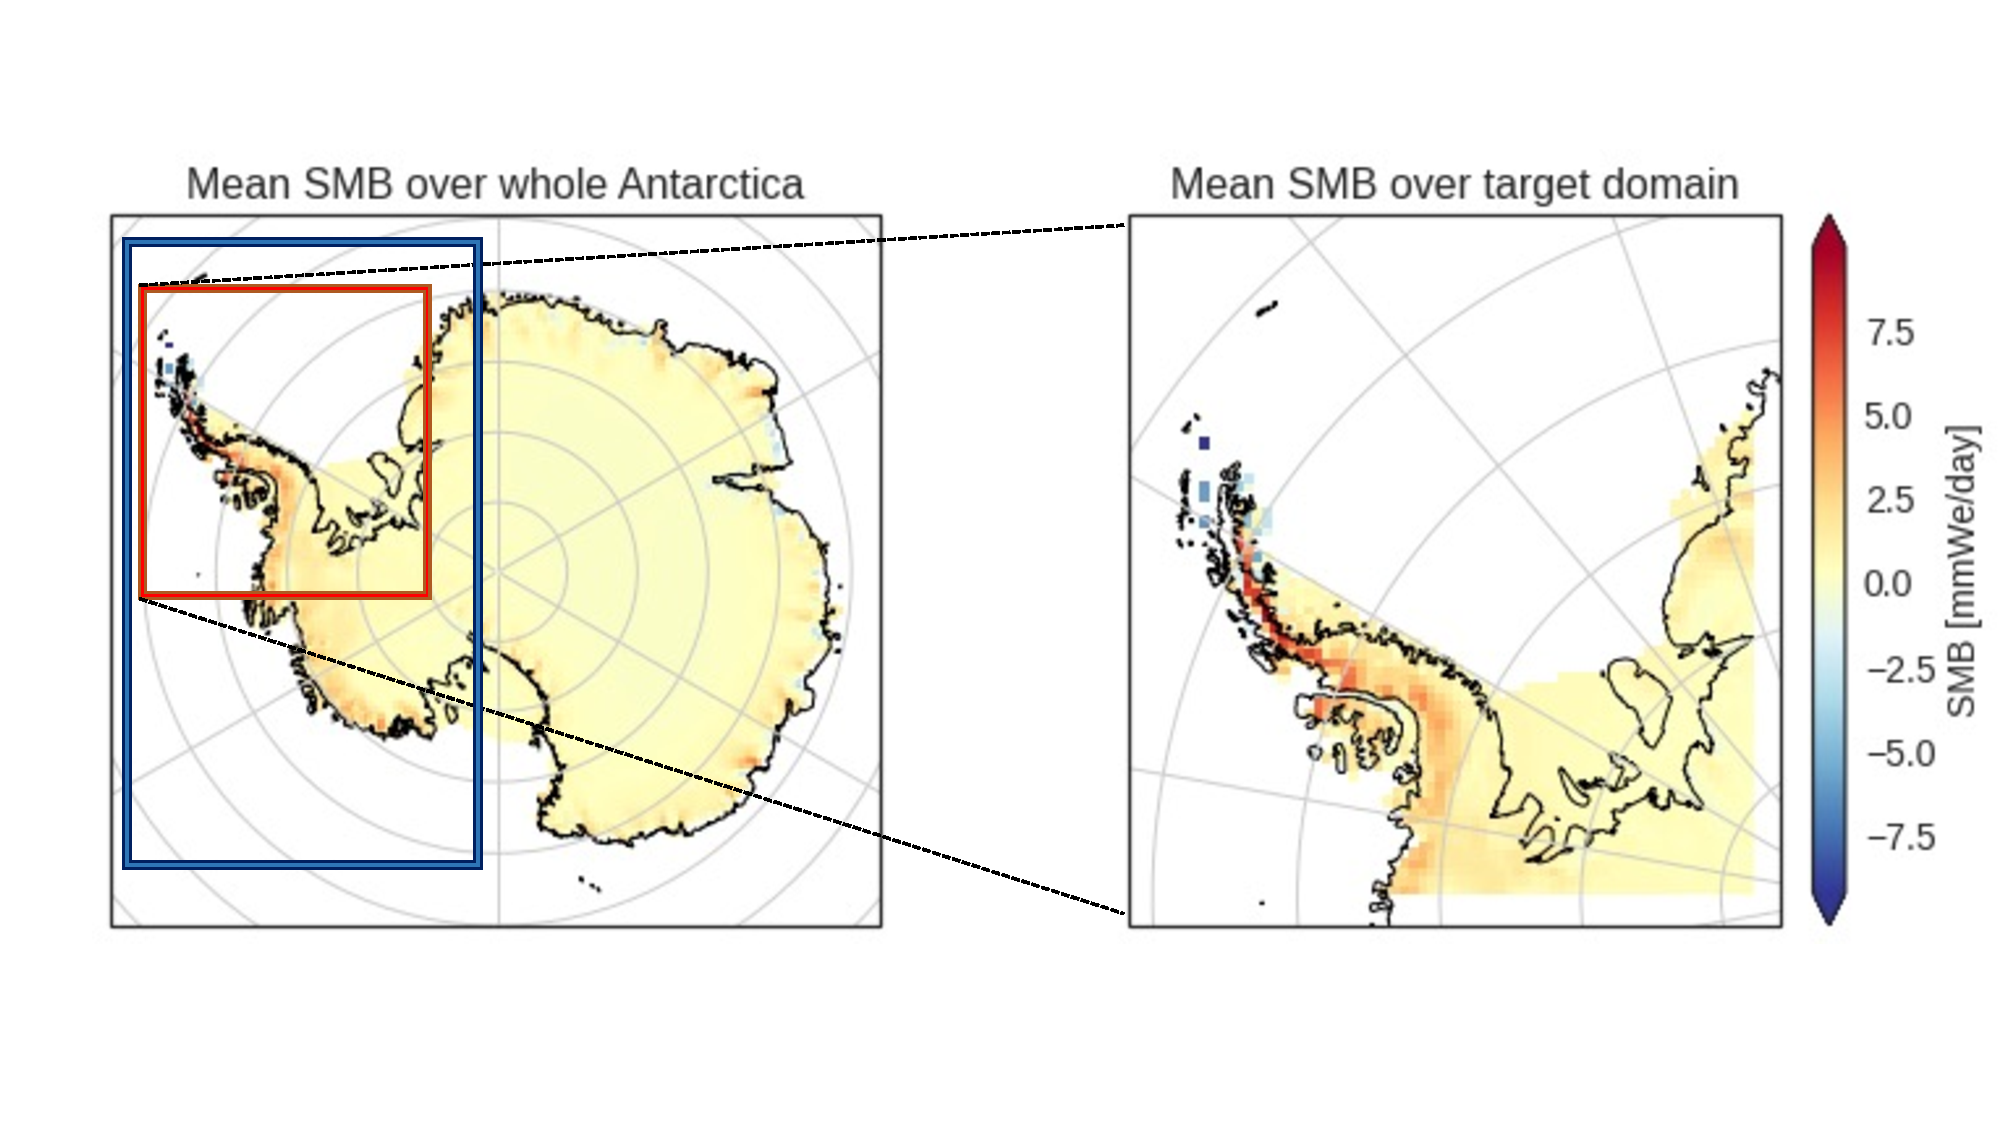
\includegraphics[width=\columnwidth]{images/domains.pdf}
  \caption []{\small Regions chosen as target domain $\mathcal{E}$ (in red) and input domain $\mathcal{D}$ (in blue) for the RCM-emulator. Illustrated underneath are the daily mean surface mass balance (SMB) over Antarctica (left) and the Antarctic Peninsula (right) from 1980 to 2100.}
  \vspace{-3mm}
    \label{fig:region-of-choice}
\end{figure}


\subsection{Target and input domain}
The target domain $\mathcal{E}$ chosen for the RCM-emulator is a grid box of $64 \times 64$ pixels at 35 \si{km} resolution that contains the Antarctic Peninsula (AP) in West Antarctica (\autoref{fig:region-of-choice}). The AP is the most northern part of Antarctica, extending over approximately 5 million square kilometers and mainly covered by ice. The region is very mountainous, with its highest peaks rising to about 3'000 \si{m} and major ice shelves on the AP include the Larsen and Ronne ice shelves. In terms of temperature, the Peninsula has the mildest climate in Antarctica. Its temperatures are warmest in January, averaging 2 $\degree C$, and coldest in June with -15 to -20 $\degree C$~\cite{AntarcticPeninsula}. Interestingly, precipitation varies significantly within the AP. The Peninsula's tip has the highest precipitation levels, with 35-50 \si{cm} per year. On the west and northeast coast, occasional precipitation leaves levels at 35 \si{cm}. On the other hand, along the east coast and the interior of Antarctica, the climate is drier, with 10-15 \si{cm}~\cite{antarctic-climate, antarctic-climate-2}. 


 Because of the specific patterns of climate variables such as temperature and precipitation, the AP has a high annual and geographical variability in SMB values. This shows when looking at mean daily SMB values (\autoref{fig:region-of-choice}). As expected from precipitation patterns, the Peninsula's tip and west coast have higher SMB values than the rest. Mean SMB values over the AP range from approximately -10 to 10 \si{mmWe/day}\footnote{millimetre water equivalent per day} while the extremes observed in this region from 1980 to 2100 are a minimum of -59 \si{mmWe/day} and a maximum of 30 \si{mmWe/day}. This variation in SMB values made this region very interesting to emulate because we wanted to see how the RCM-emulator adapted to different annual patterns of SMB over our target domain. 
 
 The input domain $\mathcal{D}$ of the RCM-emulator covers approximately 17 million square kilometers and is a $48\times25$ pixels grid box (at $68 \times 206$ \si{km} resolution) defined around the target domain. Because it is favorable to give our machine learning model a square input, it was resized to $32\times 32$ by bilinear interpolation. 



\subsection{Features}\label{subsec:features}

The RCM-emulator receives input features $(X, Z)$ that consist of two-dimensional variable $X$, and one-dimensional $Z$ (\autoref{tab:features}). $X$ is a spatial encoding of eight different atmospheric variables $x\in C_1$ measured daily at near surface level over $\mathcal{D}$. After a monthly mean aggregation of the data, the frequency of the variables becomes monthly. Each atmospheric variable at time-step $t\in T$ is normalized according to its spatial mean $\bar{X}_{t,x}$ and standard deviation $\sigma(X_{t,x})$:
\begin{equation}\label{eq:normalisation-X}
            \tilde{X}_{t,i,j,x} = \frac{X_{t,i,j,x}-\bar{X}_{t,x}}{\sigma(X_{t,x})} \;\;\;\; \forall (i,j) \in \mathcal{D}, t\in T, x\in C_1
\end{equation}
In terms of feature selection for $X$, we followed the same procedure as the authors of the temperature-emulator and used all available variables~\cite{Doury}. This gives the following equation for $X$:
\begin{equation}\label{eq:X}
    X = \left[\tilde{X}_{t\in T, x\in C_1} \right] \subset T \times \mathcal{D} \times C_1
\end{equation}


$Z$ is a one-dimensional temporal encoding that includes the time series of spatial means $\bar{X}_{t,x}$ and standard deviations $\sigma(X_{t,x})$ for each $x\in C_1$ and $t\in T$. It also includes a cosine and sine vector to encode the information about the month of the year. 

\begin{equation}
       \cos\left(\frac{2\pi t}{12}\right);\; \sin\left(\frac{2\pi t}{12}\right) \;\;\;\; \forall t\in T
\end{equation}

Overall this gives the following equation for $Z$:
\begin{equation}\label{eq:Z}
    Z = \left[ \bar{X}_{t\in T, x\in C_1}, \sigma\left(X\right)_{t\in T, x\in C_1}, \cos, \sin \right] \subset T \times C_2
\end{equation}

Each of the spatial means $\bar{X}_{t,x}$ and standard deviations $\sigma(X_{t,x})$ in Z are normalised according to a reference period ($\mathrm{ref}=$1980-2000)~\cite{Doury}:
\begin{equation}\label{eq:normalisation-Z}
    \tilde{Z}_{t,x} = \frac{Z_{t,x}-\bar{Z}_{\mathrm{\mathrm{ref}},x}}{\sigma(Z_{\mathrm{ref},x})} \;\;\;\; t\in T, x\in C_1
\end{equation}
where $\bar{Z}_{\mathrm{ref},x}$ and $\sigma(Z_{\mathrm{ref},x})$ are respectively the temporal mean and standard deviation of the spatial means or standard deviations of $X_{\mathrm{ref}, x} \subset T_{\mathrm{ref}}\times C_1$ for variable $x$. Because the $X$ variables are normalized at each time step by their spatial mean, they no longer carry any temporal encoding. Adding Z to the RCM-emulator allows it to have access to this information. 

\begin{table}[tbp]
    \centering
    \caption{}
    \renewcommand\arraystretch{1.5}
    \begin{tabular}{l>{\centering}p{0.1\linewidth}>{\centering}p{0.2\linewidth}>{\centering\arraybackslash}p{0.2\linewidth}}
    \toprule
        \textbf{Variable Name} & \textbf{Variable Notation} & \textbf{Units} & \textbf{Dimensions} \\ \toprule
        \textbf{2D variables} & & & \\ \bottomrule 
        Northward Wind & NW & $[ms^-1]$ & $ \mathcal{D}$   \\ 
        Eastward Wind & EW & $[ms^-1]$ & $ \mathcal{D}$ \\
        Downwelling Shortwave Radiation & SWD & $[Wm^{-2}]$ & $ \mathcal{D}$ \\
        Downwelling Longwave Radiation & LWD & $[Wm^{-2}]$ & $ \mathcal{D}$ \\
        Specific Humidity & QQP & $[g/Kg]$ & $ \mathcal{D}$ \\
        Temperature & TT & $[\degree]$ & $ \mathcal{D}$ \\
        Precipitation & PR & $[mmWe/day]$ & $ \mathcal{D}$  \\
        Pressure & PR & $[hPa]$ & $ \mathcal{D}$  \\
        \toprule
         \textbf{1D variables} & & & \\ \bottomrule
        Spatial mean of 2D variables & $\bar{X}_{x}$ & & $[C_1]$ \\ 
        Spatial std of 2D variables & $\sigma\left(X_{x}\right)$ & & $[C_2]$ \\
        Seasonal Indicators & & & $[2]$\\ \bottomrule
        
    \end{tabular}
        \subcaption*{\small Table~\ref{tab:features}. Two and one-dimensional input features given to the model. Each feature is measured (near) surface and a monthly mean aggregation.}
            \label{tab:features}
\end{table}

\section{Model}\label{sec:model}

\begin{figure}[!t]
  \centering
  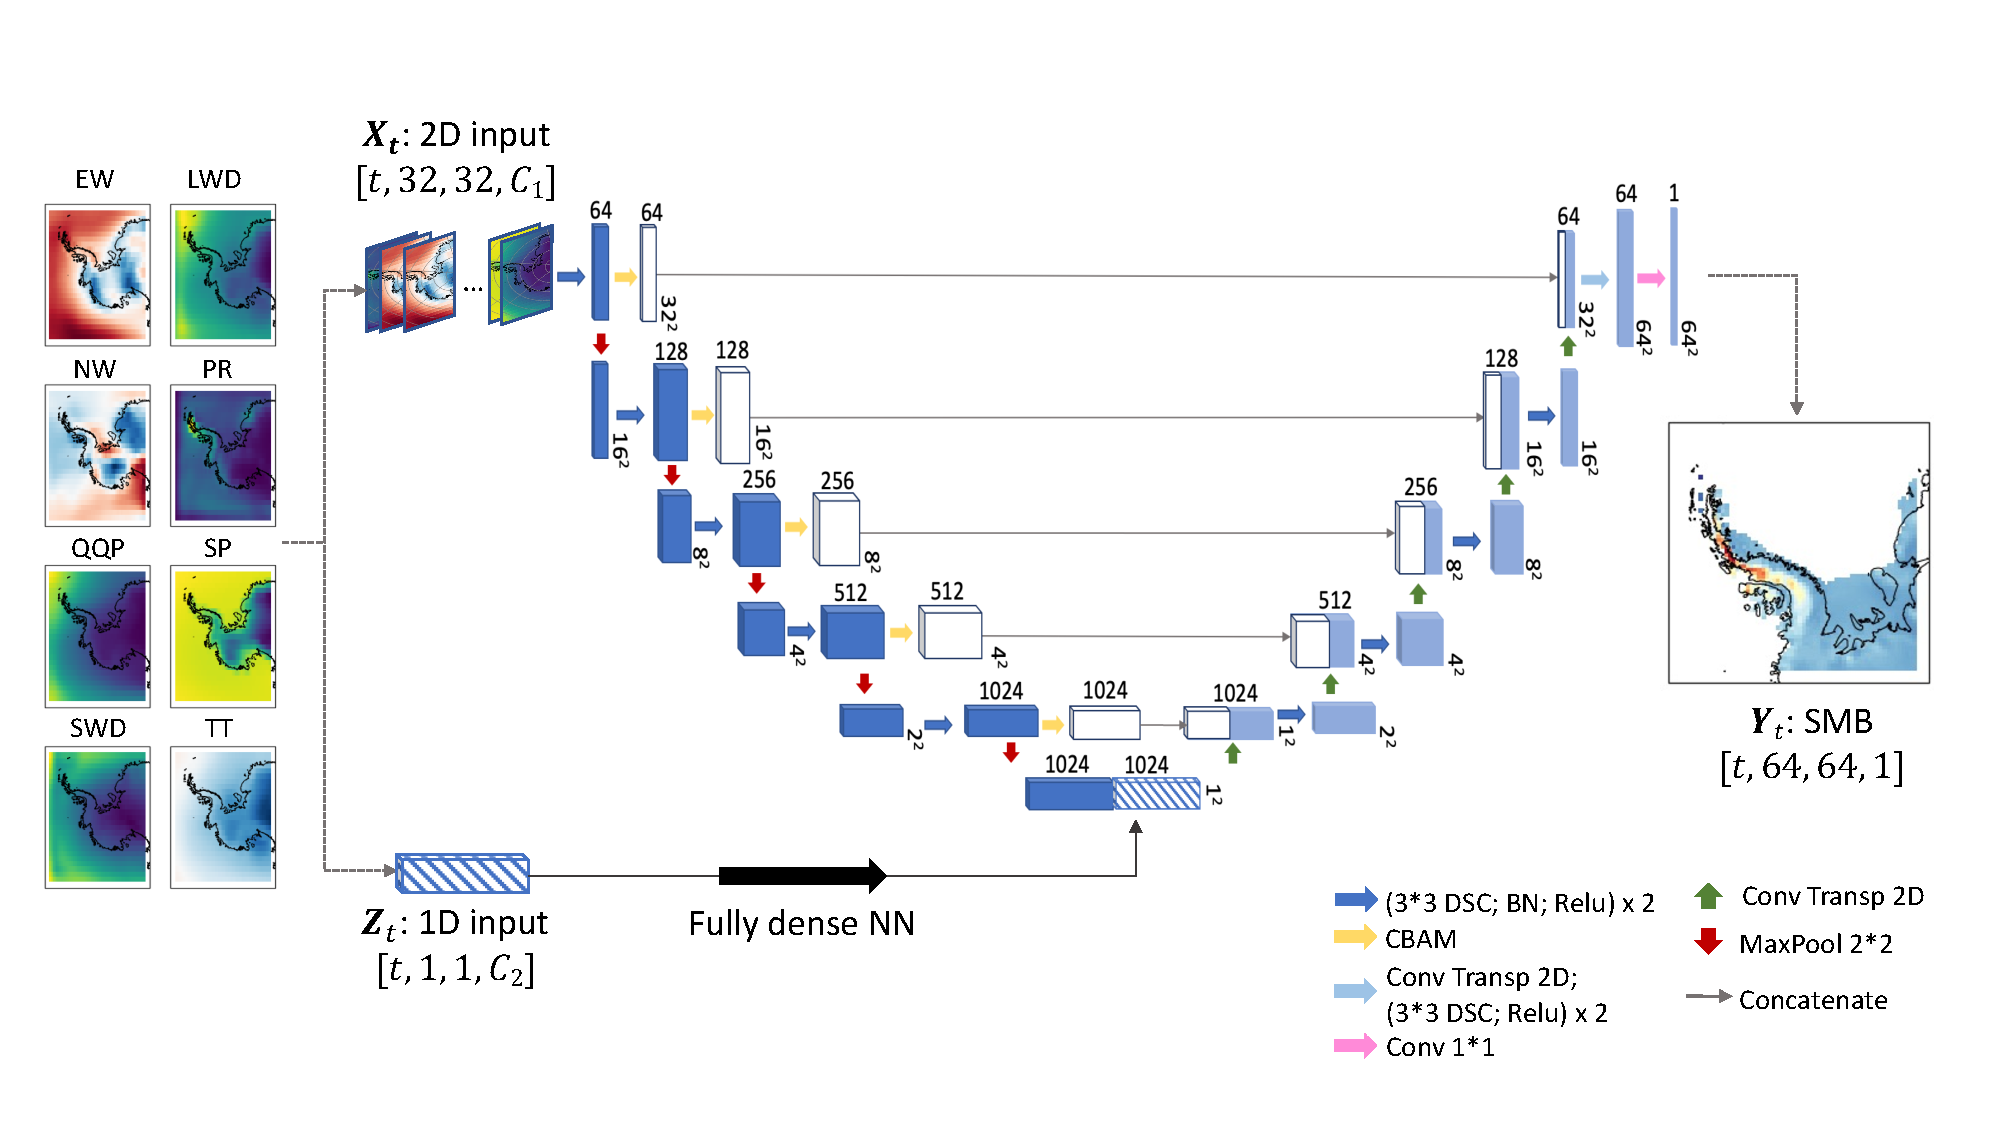
\includegraphics[width=\columnwidth]{doc/Thesis-latex/images/unet-with-data.pdf}
  \caption []{\small Illustration of an observation at time-step $t$. Left: 2D input variables $X_t$ on the input domain with its corresponding 1D variable $Z_t$. Right: target surface mass balance (SMB) $Y_t$ on the target domain. Middle: scheme of the U-Net architecture used for this paper.}
  \vspace{-3mm}
  \label{fig:example-features}
\end{figure}

\subsection{Architecture}\label{subsec:architecture}
Our emulator's architecture extends the traditional U-Net~\cite{unet} used to emulate near-surface temperature in~\cite{Doury} with mechanisms from the SmaAt-UNet model~\cite{smatunet} (\autoref{fig:example-features}). The SmaAt-UNet equips the U-Net architecture with convolutional block attention mechanisms (CBAM) and depthwise-separable convolutions (DSC) instead of regular convolutional operations.

The network is U-shaped, divided into a down-sampling (encoder) section that forms the left side and an up-sampling (decoder) on the right. The encoder consists of double convolutions (blue arrow in \autoref{fig:example-features}) followed by max-pooling (red arrow). This process halves the image size and doubles the number of channels at each layer of the U-Net. Instead of traditional convolutional operations, the emulator uses DSC, designed to reduce the number of parameters and make the model faster~\cite{smatunet}. 

At the bottom of the U-Net, encoded spatial information from $X_t$ and temporal information from $Z_t$ are concatenated. The corresponding 1D input $Z_t$ of $X_t$ first goes through a fully dense neural network to reach the same number of channels as the output of the last layer of the encoder. Then, it is concatenated with the encoder output at the bottom of the "U". This constrains the U-Net to give equal importance to the spatial and temporal inputs before starting the decoding path and generating the high-resolution SMB image~\cite{Doury}. 

The decoder is built out of three parts. First, a 2D transposed convolution operation (green arrow) doubles the image size. Then, the resulting feature maps are concatenated with the previous encoder's attention maps (white block) via skip-connections (grey arrow). Lastly, a double depthwise-separable halves the number of channels (blue arrow). Skip-connections between layers (grey arrow) make it possible to skip large sections if required and create a smoother loss surface~\cite{Li2017}. An additional up-sampling layer (light blue arrow) is added to the decoder to reach the target size ($64\times 64$), and a $1\times1$ convolution (pink arrow) changes the number of channels from 64 to 1. The model outputs a single image representing the SMB values predicted by the network at time-step $t$.

Convolutional block attention modules (yellow arrow) are placed after each double convolution in the encoder and used to detect important features over the channels and spatial regions of the inputs~\cite{smatunet}. In CBAMs, the attention mechanism is first applied over the channels of the image and then the spatial dimension. Note that the input to the next layer of the encoder is not the attention feature map (white block) but the convoluted and downsampled image of the previous layer (dark blue block). This way, the original image features are preserved throughout the encoder layers. The attention blocks are fed through skip-connections to the corresponding decoder layer to be concatenated. Contrary to the DSC convolutions used in the encoder and decoder, CBAMs use regular convolutions.  

\subsection{Perfect model framework}\label{subsec:perfect-model}

We were inspired by the \textit{perfect model framework} from~\cite{Doury} where both the low-resolution inputs and high-resolution target SMB come from the same RCM simulation when training the emulator. In this setting, the model aims to learn only the downscaling function $F$ of the RCM (\autoref{eq:emulator-equation}). For this, it needs perfect consistency i.e., high temporal and spatial correlation, between the global-scale inputs and the regional-scale target. Otherwise, the emulator will try to learn a relationship between them that does not exist or is imprecise~\cite{Doury}. Because of large-scale biases and inconsistencies between GCM and RCM variables, a perfect consistency cannot be guaranteed~\cite{Sanchez2009, Sanchez2018}. The perfect model framework provides it.

To test the effect of this perfect model training framework on our SMB-emulator, we created "GCM-like" features from the RCM ($\operatorname{UPRCM}$). First, we used conservative interpolation to upscale RCM features to GCM resolution ($68\times206$ km). Then, the upscaled RCM features were smoothed with a $3\times3$ moving average filter. This filter conserves the GCM grid while smoothing out the information of each pixel. This further ensured the removal of local-scale information that might remain after the upscaling~\cite{Doury, Klaver2020}.


To assess the presence of biases and inconsistencies between UPRCM and GCM features, we used two correlation statistics:  
\begin{itemize}
        \item Temporal correlation: for each atmospheric variable $x\in C_1$ and point $p = (i,j)$ in the input domain $\mathcal{D}$, we calculated the Pearson correlation coefficient between the GCM and UPRCM time series:
        \begin{equation}\label{eq:temporal-corr}
            \rho\left(G_{p}^x,U_{p}^x\right) = \frac{\operatorname{cov}(G_{p}^x,U_{p}^x)}{\sigma(G_{p}^x)\sigma(U_{p}^x)} \;\;\;\; \forall p \in \mathcal{D}, x\in C_1 
        \end{equation}
        where $G_{p}^x = \operatorname{GCM}[1:T, i, j, x]$, $U_{p}^x = \operatorname{UPRCM}[1:T, i, j, x]$, $\operatorname {cov}(\cdot)$  is the covariance and  $\sigma(\cdot)$ is the standard deviation.  
        \item Spatial correlation: for each $x\in C_1$ and time-step $t \in T$, we calculated the spatial correlation between GCM and UPRCM images: 
        \begin{equation}\label{eq:spatial-corr}
            \operatorname{sc}\left(G_{t}^x,U_{t}^x\right) = \frac{\operatorname{cov}(G_{t}^x,U_{t}^x)}{\sigma(G_{t}^x)\sigma(U_{t}^x)} \;\;\;\; \forall t \in T, x\in C_1 
        \end{equation}
        where $G_{t}^x = \operatorname{GCM}[t,1:I,1:J,x]$ and $U_{t}^x =\operatorname{UPRCM}[t,1:I,1:J,x]$. 
    \end{itemize}


\section{Training}\label{subsec:training}
As aforementioned in~\autoref{subsec:features}, each single observation given to our emulator is composed of features $X_t$ and $Z_t$ for a month $t\in T$. $X_t$ is an array in $I \times J \times C_1$, where the two first dimensions are the spatial size of the input domain, and the number of channels $C_1$ is the different atmospheric variables chosen as predictors. $Z_t \subset C_2$ is its corresponding temporal encoding (\autoref{fig:example-features}).


We created two emulators by following two scenarios. We trained the first emulator ($\mathrm{\hat{F}_U}$) following the perfect model framework (\autoref{subsec:perfect-model}) where we used UPRCM features as low-resolution inputs. Then, in a second step, we trained another emulator ($\mathrm{\hat{F}_G}$) with coarse features directly from the GCM. The perfect model framework allowed us to evaluate how the U-Net performs when it has to learn only the downscaling function of the RCM. In the second training setting, we wanted to see whether the model could learn the underlying dynamics, despite inconsistencies and biases, between GCM and RCM. 


In the temperature-emulator from~\cite{Doury}, the authors propose to view the problem as a regression and use MSE as a loss function. However, our emulator performed poorly using an MSE loss, and it did not seem appropriate to our setting. As aforementioned, the scale of SMB values varies significantly across the target domain of the Antarctic Peninsula. For example, dry inland points have small annual variations of SMB, with maximum values reaching under 2 \si{mmWe/day}, while a point on the west coast of the Peninsula can reach low extremes of -20 \si{mmWe/day}. In this unbalanced setting, MSE penalizes the ill-fitting of low SMB regions less than points with high values of SMB. For this reason, we chose to use a normalized RMSE (NRMSE) loss. Normalizing the RMSE facilitates comparing datasets with different magnitude scales, as in our case. For each observation i.e., each time step $t$, given to the emulator, we calculated the NRMSE loss between the predicted SMB maps $\hat{Y}^{t}$ and the true $Y^{t}$ over all positions $p \in \mathcal{E}$:
\begin{align*}
        \operatorname{NRMSE}\left(Y^{t},\hat{Y}^{t}\right) &= \frac{\operatorname{RMSE}}{Y_{\max} - Y_{\min}} \\
         &=\frac{\sqrt{\frac{1}{P}\sum_{p}(\hat{y}_{p}^{t}-y^{t}_{p})^2}}{Y_{\max} - Y_{\min}}   \;\;\;\; \forall t \in T
\end{align*}
where $\hat{y}_{p}^{t}$ is the SMB value predicted at location $p$ and time $t$, $P$ the number of points in $\mathcal{E}$ and $Y_{\max}$, $Y_{\min}$ are respectively the maximum and minimum value of SMB over $T$ and $\mathcal{E}$.

We trained both emulators using a batch size of 100 and over 50 epochs. We used early stopping and a learning-rate scheduler that reduced the learning rate on loss plateaus ($\operatorname{LR}_0 = 0.005$). 

The RCM-emulator architecture was implemented in PyTorch 1.11 and is available on our \href{https://github.com/marvande/master-thesis}{GitHub}. Training was done on Google Colab's GPU (NVIDIA Tesla K80).

\section{Evaluation}\label{sec:evaluation}

% evaluation framework
\begin{figure}[!t]
  \centering
  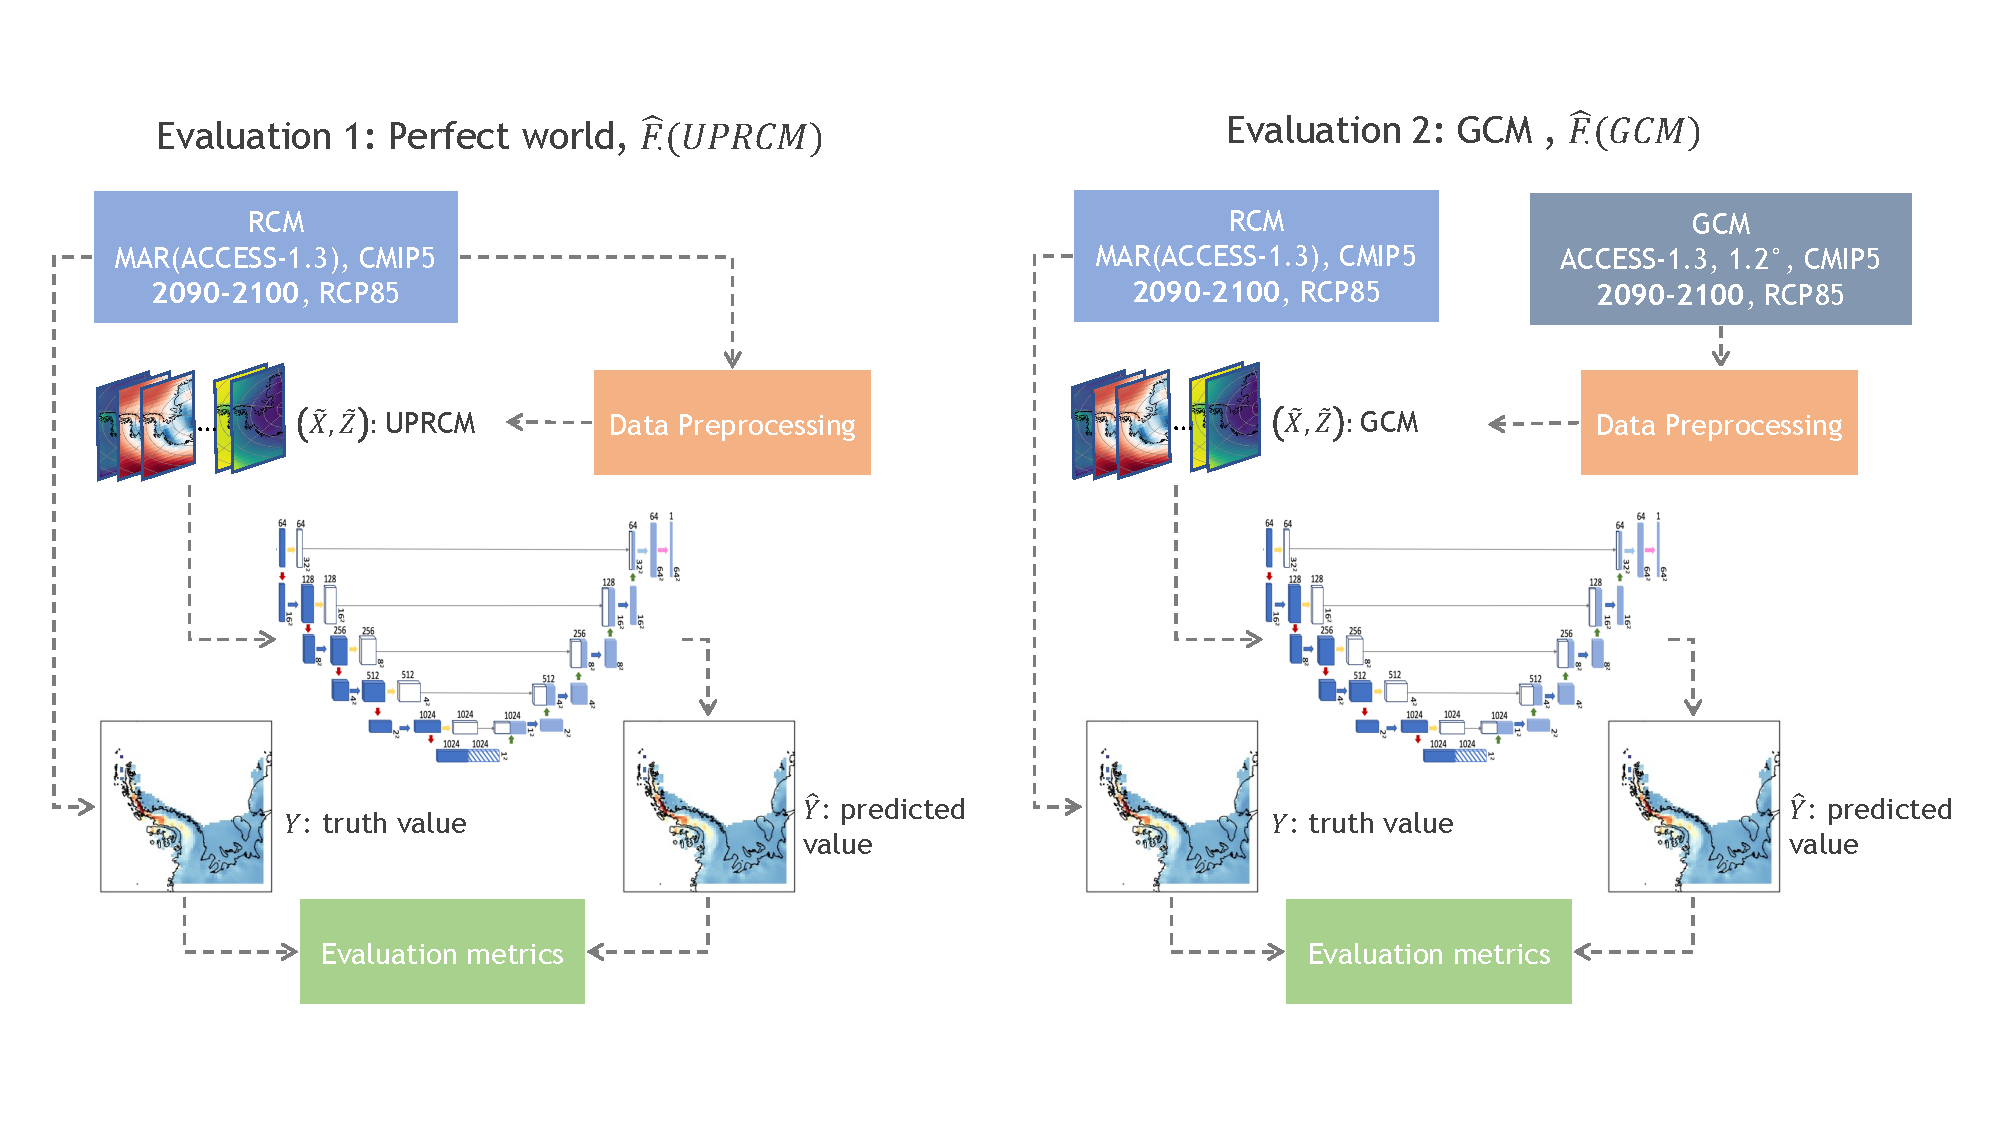
\includegraphics[width=\columnwidth]{doc/Thesis-latex/images/evaluation_framework.pdf}
  \caption []{\small Evaluation frameworks of the RCM-emulator. Left: perfect world scenario where the emulator $\mathrm{\hat{F}_{U}}$ or $\mathrm{\hat{F}_{G}}$ makes regional SMB predictions using upscaled RCM features (UPRCM) as global-scale inputs - $\mathrm{\hat{F}_{\cdot}(UPRCM)}$. Right: global-scale features come from the GCM for predictions - $\mathrm{\hat{F}_{\cdot}(GCM)}$. Evaluation metrics used to compare predictions and the true SMB truth are described in~\autoref{subsec:evaluation-metrics}.}
  \vspace{-3mm}
  \label{fig:evaluation-framework}
\end{figure}

We separated the time-frame $T$ of the climate simulations into an approximate 90\%-10\% split with a train and test period of $T_{train} = 1980-2090$ and $T_{test} = 2090-2100$, so that the RCM-emulator made predictions on features never seen during training. We arbitrarily chose to put the test period at the end of the climate model's time frame out of simplicity, but we could also have taken the test samples elsewhere as long as they were consecutive. 
\subsubsection{Evaluation of $\mathrm{\hat{F}_U}$}

To inspect how the emulator performs under conditions similar to those of its training, we first evaluated emulator $\mathrm{\hat{F}_U}$ in the perfect model with UPRCM features - $\mathrm{\hat{F}_U(UPRCM)}$. Then, in a second step, we evaluated the emulator on GCM inputs, $\mathrm{\hat{F}_U(GCM)}$. This assessed how the emulator trained on UPRCM could apply what it learned to GCM features. Furthermore, the performance of $\mathrm{\hat{F}_U(GCM)}$ is also a good indicator of the presence of inconsistencies between UPRCM and GCM features. 

\subsubsection{Evaluation of $\mathrm{\hat{F}_G}$}
 Because we trained this emulator on the GCM, we evaluated $\mathrm{\hat{F}_G}$ directly on test features from the GCM - $\mathrm{\hat{F}_G(GCM)}$.

The two evaluation frameworks are illustrated in \autoref{fig:evaluation-framework}. For each emulator $\mathrm{\hat{F}_{\cdot}}$, we assessed single month and average predictions made over the target domain. This way, we could examine which regions of the Antarctic Peninsula had the best reconstruction of SMB patterns in terms of details, precision, and intensity. Furthermore, we looked at individual time series of predicted SMB values for single points in the target region. We specifically chose these points to evaluate how the model handled different patterns and intensities of SMB.  

\subsection{Evaluation metrics}\label{subsec:evaluation-metrics} 

To evaluate the global performance of our machine learning model, we used different traditional statistics. For each RCM-emulator $\mathrm{\hat{F}}$ and point $p \in \mathcal{E}$, we compared the target SMB time series $Y_{p}$ to the predicted values $\widehat{Y_{p}}$ over the time period $T_{test}$ (2090-2100). We used the Pearson correlation coefficient, RMSE, and Wasserstein distance as evaluation metrics. Correlation is a good indicator of the reconstruction of temporal patterns such as global synchrony and seasonality. RMSE and the Wasserstein distance evaluate the fitting of extreme values and the representation of monthly variability. 

\subsubsection{Pearson correlation coefficient}\label{subsubsec:pearson-corr}
The Pearson correlation coefficient measures how two continuous time series change over time as a number between -1 (negatively correlated), 0 (uncorrelated), and 1 (perfectly correlated)~\cite{Pearson}.
\begin{equation}
    \operatorname{r}\left(Y_{p},\widehat{Y_{p}}\right) = \frac{\operatorname{cov}(Y_{p},\widehat{Y_{p}})}{\sigma(Y_{p})\sigma(\widehat{Y_{p}})} \;\;\;\; \forall p \in \mathcal{E} 
\end{equation}
where $\operatorname {cov}(\cdot)$  is the covariance and  $\sigma(\cdot)$ is the standard deviation.

\subsubsection{RMSE}\label{subsubsec:rmse}
Root Mean Squared Error (RMSE) measures the square root of the average squared differences between predicted and target observations. It is also defined as the square of the MSE:
\begin{align}\label{eq:RMSE}
        \operatorname{RMSE}\left(Y_{p},\widehat{Y_{p}}\right) & = \sqrt{\operatorname{MSE}\left(Y_{p},\widehat{Y_{p}}\right)} \\ & = \sqrt{\frac{1}{T_{test}}\sum_{t}(\hat{y}_{p}^{t}-y^{t}_{p})^2} & \forall p \in \mathcal{E} 
\end{align}
where $\hat{y}_{p}^{t}$ is predicted SMB value and $y^{t}_{p}$ the true SMB value at location $p\in \mathcal{E} $ and time step $t\in T_{test}$. 

\subsubsection{Wasserstein distance}\label{subsubsec:wasserstein}
The Wasserstein distance measures the distance between two probability density functions $f(\cdotp)$, in our case $f(Y_p)$ and $f(\widehat{Y_p})$. It is the numerical cost of an optimal transportation problem i.e., the cost of the optimal transport plan~\cite{villani} for moving the mass in the predicted
measure to match that in the target~\cite{wasserstein1}. 
\begin{equation}
    \operatorname{W}\left(f(Y_p),f(\widehat{Y_p})\right) = \sum_{t}|y^{t}_{p}-\hat{y}_{p}^{t}| \;\;\;\; \forall p \in \mathcal{E}
\end{equation}
where $\hat{y}_{p}^{t}$ is the predicted SMB value and $y^{t}_{p}$ the true SMB value at location $p\in \mathcal{E} $ and time step $t\in T_{test}$. 

\begin{comment}
 \subsection{Feature importance}\label{subsec:feature-importance}
\begin{itemize}
    \item For each emulator $\hat{F}_{(\cdot)}$, we were interested in exploring which atmospheric variables had the biggest impact on the performance of the models.
    \item Neural Networks have a reputation of being a black box algorithm with a decision process that is hard to understand. Nevertheless, there are ways to evaluate the importance of features, such as permutation importance. 
    \item Permutation importance is calculated after a model has been fitted. For each single variable in the data, its content are shuffled i.e, rendering the images unreadable and then the model's performance is evaluated with that corrupted variable.
    \item For every variable $x\in C_1$ in the test dataset $X[1:T_{test}, 1:I,1:J,1:C_1]$, we computed the difference between the prediction score on the original data and that of corrupted features. This procedure was repeated $K$ times and the importance was calculated as the mean percentage of difference in scores. 
    \begin{equation}
        \operatorname{I_x} =\frac{1}{K}\sum_{k\in K} \frac{100*(\operatorname{s}_{x}^k - \operatorname{s})}{\operatorname{s}} \;\;\; \forall x\in C_1    \end{equation}
    where $s$ is the NRMSE loss on the original prediction of $\hat{F}_{(\cdot)}$ and $s_x^k$ is the loss for repetition $k\in K$ and corrupted feature $x\in C_1$. 
    \item What is expected: 
    \begin{itemize}
    \item With this technique, we expected to obtain less precise predictions for corrupted features because the resulting data no longer conforms to anything observed by the emulators~\cite{FeatureImportance2}.
    \item Why? This method breaks the relationship between the features and the target. Because we corrupted the natural structure of the data with our scrambling, we compromised what our model learned during training, resulting in higher errors. Hence the drop in the model score is an indication of how much the model depends on the feature.~\cite{FeatureImportance}
    \end{itemize}
    \item Note that: 
    \begin{itemize}
        \item Permutation importance is not a reflection of the actual predictive value of a feature per se but rather the significance of that feature to a specific model.~\cite{FeatureImportance2}
        \item If two features are correlated and one of them is permuted, the model still has access to this feature via the correlated one. This leads to lower importance for both features, although they might actually be important.~\cite{FeatureImportance2}. 
    \end{itemize}
\end{itemize}
\end{comment}

\chapter{Results}
%%%%%%%%%%%%%%%%%%%%

\section{Prediction maps}\label{subsec:geoplots}
To evaluate the performance of our RCM-emulator at reconstructing spatial structures of SMB values, we compared a prediction for a random month and the average predictions over the test period to the RCM truth. Prediction maps are compared to the truth using RMSE and results can be seen in \autoref{fig:geoplots-GCM-RCM}. 

Unsurprisingly, in the first two columns in \autoref{fig:geoplots-GCM-RCM}, we see that compared to the low-resolution UPRCM map, the high-resolution RCM truth is more detailed and has a more complex spatial structure. As expected, because of their precipitation patterns, we see that the tip and west coast of the Antarctic Peninsula show high values of SMB in the RCM truth, some points reaching 10 \si{mmWe/day}. For the chosen random month of May 1980, except for higher intensity regions in the mainland, both $\mathrm{\hat{F}_{U}(UPRCM)}$ and $\mathrm{\hat{F}_{G}(GCM)}$ competently reproduce the spatial structure of the RCM truth. On average, both emulators' predictions also look very similar to the average true SMB. The emulators have a very small RMSE (0.27 and 0.30), which becomes even smaller when looking at the average prediction over the test period (0.09 and 0.08). On the other hand, $\mathrm{\hat{F}_{U}(GCM)}$, both for the random month and on average, is not able to reproduce the extreme values of SMB and creates a toned-down version of the truth. In particular, it underestimates the high magnitude SMB values on the west coast of the Antarctic Peninsula. This is reflected in its RMSE, which is twice as high as the other two models (0.53 for a random month and 0.23 on average). 

Overall, these results hint that both emulators $\mathrm{\hat{F}_{U}}$ and $\mathrm{\hat{F}_{G}}$, when evaluated on data similar to what they were trained on, have a solid capacity to reproduce the complex spatial structures of the RCM. 



% SMB predictions over geoplots
\begin{figure}[thb]
  \centering
  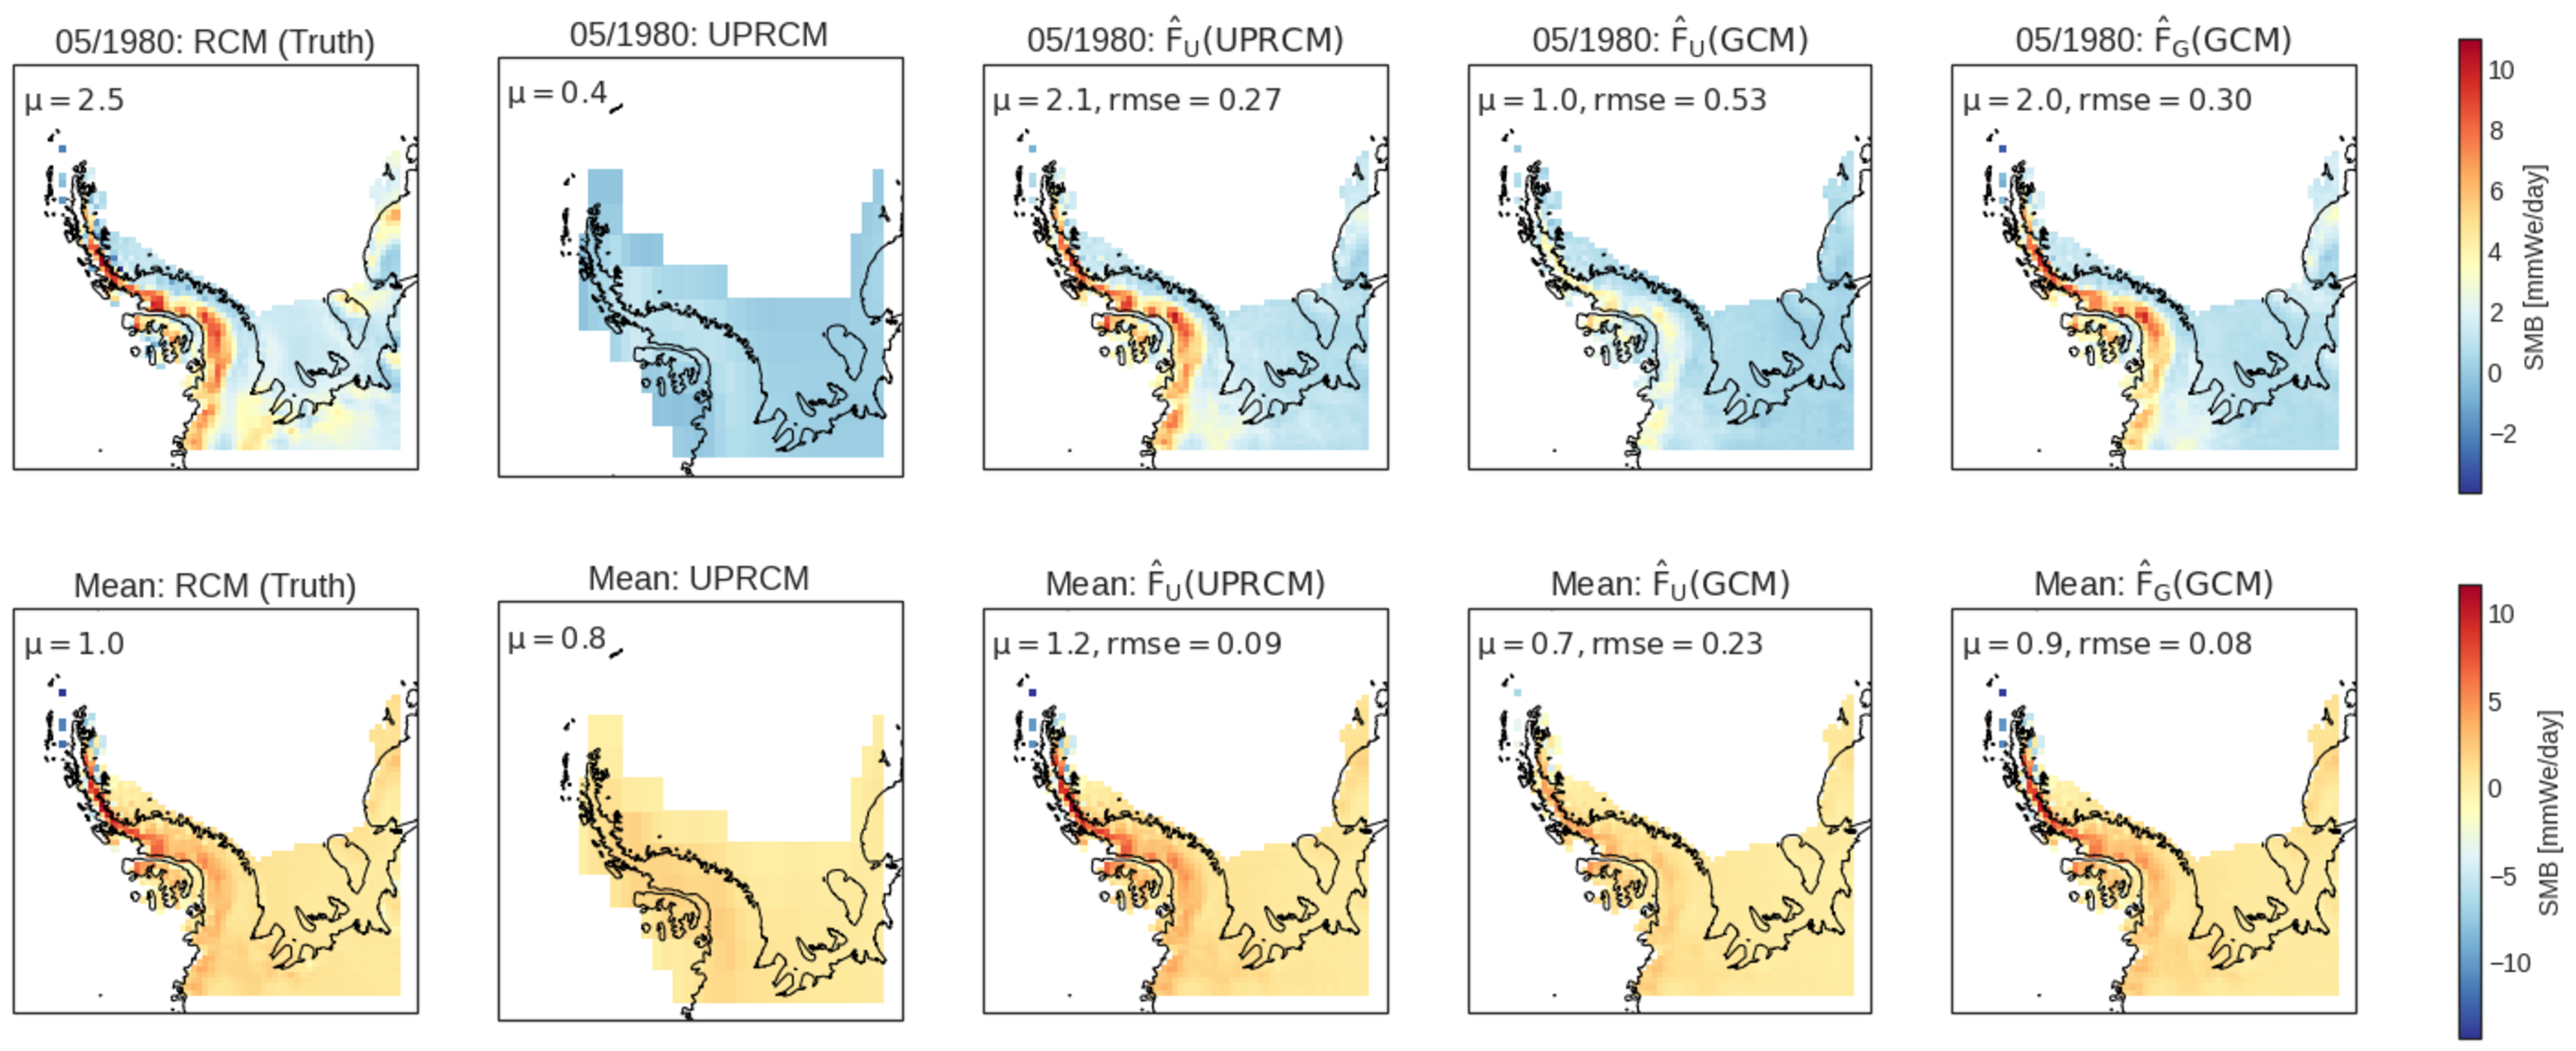
\includegraphics[width=\columnwidth]{doc/Thesis-latex/images/results/geoplots_RCM_GCM.pdf}
  \caption []{\small Surface mass balance (SMB) predictions of the RCM-emulator on a random month (05/1980) (top) and averaged over the test period (2090-2100) (bottom) over target domain $\mathcal{E}$. From left to right: SMB in RCM truth, UPRCM, $\mathrm{\hat{F}_{U}(UPRCM)}$, $\mathrm{\hat{F}_{U}(GCM)}$ and $\mathrm{\hat{F}_{G}(GCM)}$. Legend: spatial mean ($\mu$) of SMB over $\mathcal{E}$ and spatial RMSE ($\mathrm{rmse}$) between the emulated and true RCM SMB pixel values.}
  \vspace{-3mm}
  \label{fig:geoplots-GCM-RCM}
\end{figure}

\section{Time-series of predictions}\label{sec:res-time-series}
To assess how the RCM-emulator can predict different temporal patterns and intensities of SMB, we plotted the emulated time series for four geographical points (\autoref{fig:points-location}). P1 on the Larsen Ice Shelf has high precipitation levels, and SMB values oscillate annually between -5 and 5 \si{mmWe/day}. P2 on the west coast, has SMB values reaching low extremes of -15 \si{mmWe/day}. P3 on the east coast has low yearly precipitation and minor SMB variations (0-4 \si{mmWe/day}). P4 on the Ronne ice shelf, has a significantly drier climate (0-1.5 \si{mmWe/day}). \autoref{fig:timeseries-GCM-UPRCM} presents each point's time series and annual SMB predictions. For each point, the RMSE, NRMSE, and Pearson correlation coefficient are calculated between the predicted and true SMB time series. 

For each of these four points, $\mathrm{\hat{F}_{U}(UPRCM)}$ and $\mathrm{\hat{F}_{G}(GCM)}$ come very close to reproducing the temporal patterns of the RCM truth series, as is expected from the results of \autoref{subsec:geoplots}. For P1 and P2, all emulators reproduce seasonality well, with high correlation values to the true SMB (close to 1 for P2). $\mathrm{\hat{F}_{G}(GCM)}$ is even a little bit better than $\mathrm{\hat{F}_{U}(UPRCM)}$ at emulating low drops and high peaks in SMB. For P3 and P4, both emulators show a good ability to reproduce the time series pattern, even when their behavior is less seasonal, like for P3. We notice for P4, that the emulators have difficulties reproducing multiple close peaks per year and tend to merge them into one prominent peak. 


As was already seen in \autoref{fig:geoplots-GCM-RCM}, $\mathrm{\hat{F}_{U}(GCM)}$ tends to underestimate high amplitude values of SMB, and this is noticeable in the time series for all four points. The $\mathrm{\hat{F}_{U}(GCM)}$ predictions can reproduce the seasonal patterns (reflected in a high correlation) but produce a toned-down version of the true RCM time series (mirrored in a higher RMSE). This is observable also in the time series' distributions, where the peak of $\mathrm{\hat{F}_{U}(GCM)}$ is higher and centered around lower SMB values compared to $\mathrm{\hat{F}_{U}(UPRCM)}$ and $\mathrm{\hat{F}_{G}(GCM)}$, which are more spread out and closer to the RCM truth. This pattern repeats in the annual SMB predictions for all emulators. $\mathrm{\hat{F}_{U}(UPRCM)}$ and $\mathrm{\hat{F}_{G}(GCM)}$ come very close to the true annual SMB values, with $\mathrm{\hat{F}_{G}(GCM)}$ again slightly better than $\mathrm{\hat{F}_{U}(UPRCM)}$ for almost all years. $\mathrm{\hat{F}_{U}(GCM)}$ on average consistently underestimates the truth by a factor of 2. 


% Time series and geoplots for four points
\begin{figure}[!h]
        \centering
        \begin{subfigure}[b]{0.2\columnwidth}
            \centering 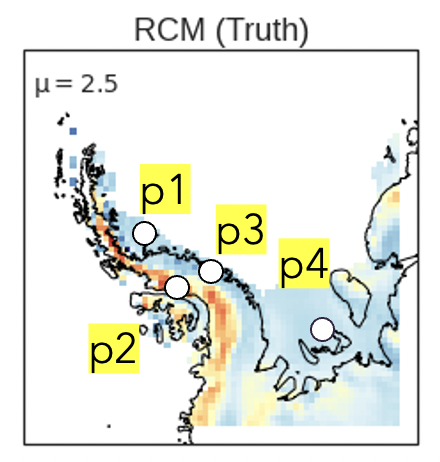
\includegraphics[width=\textwidth]{doc/Thesis-latex/images/results/points_location.png}
            \caption[]%
            {{\small}}    
          \label{fig:points-location}
        \end{subfigure}
        \hfill
        \begin{subfigure}[b]{\columnwidth}  
            \centering 
           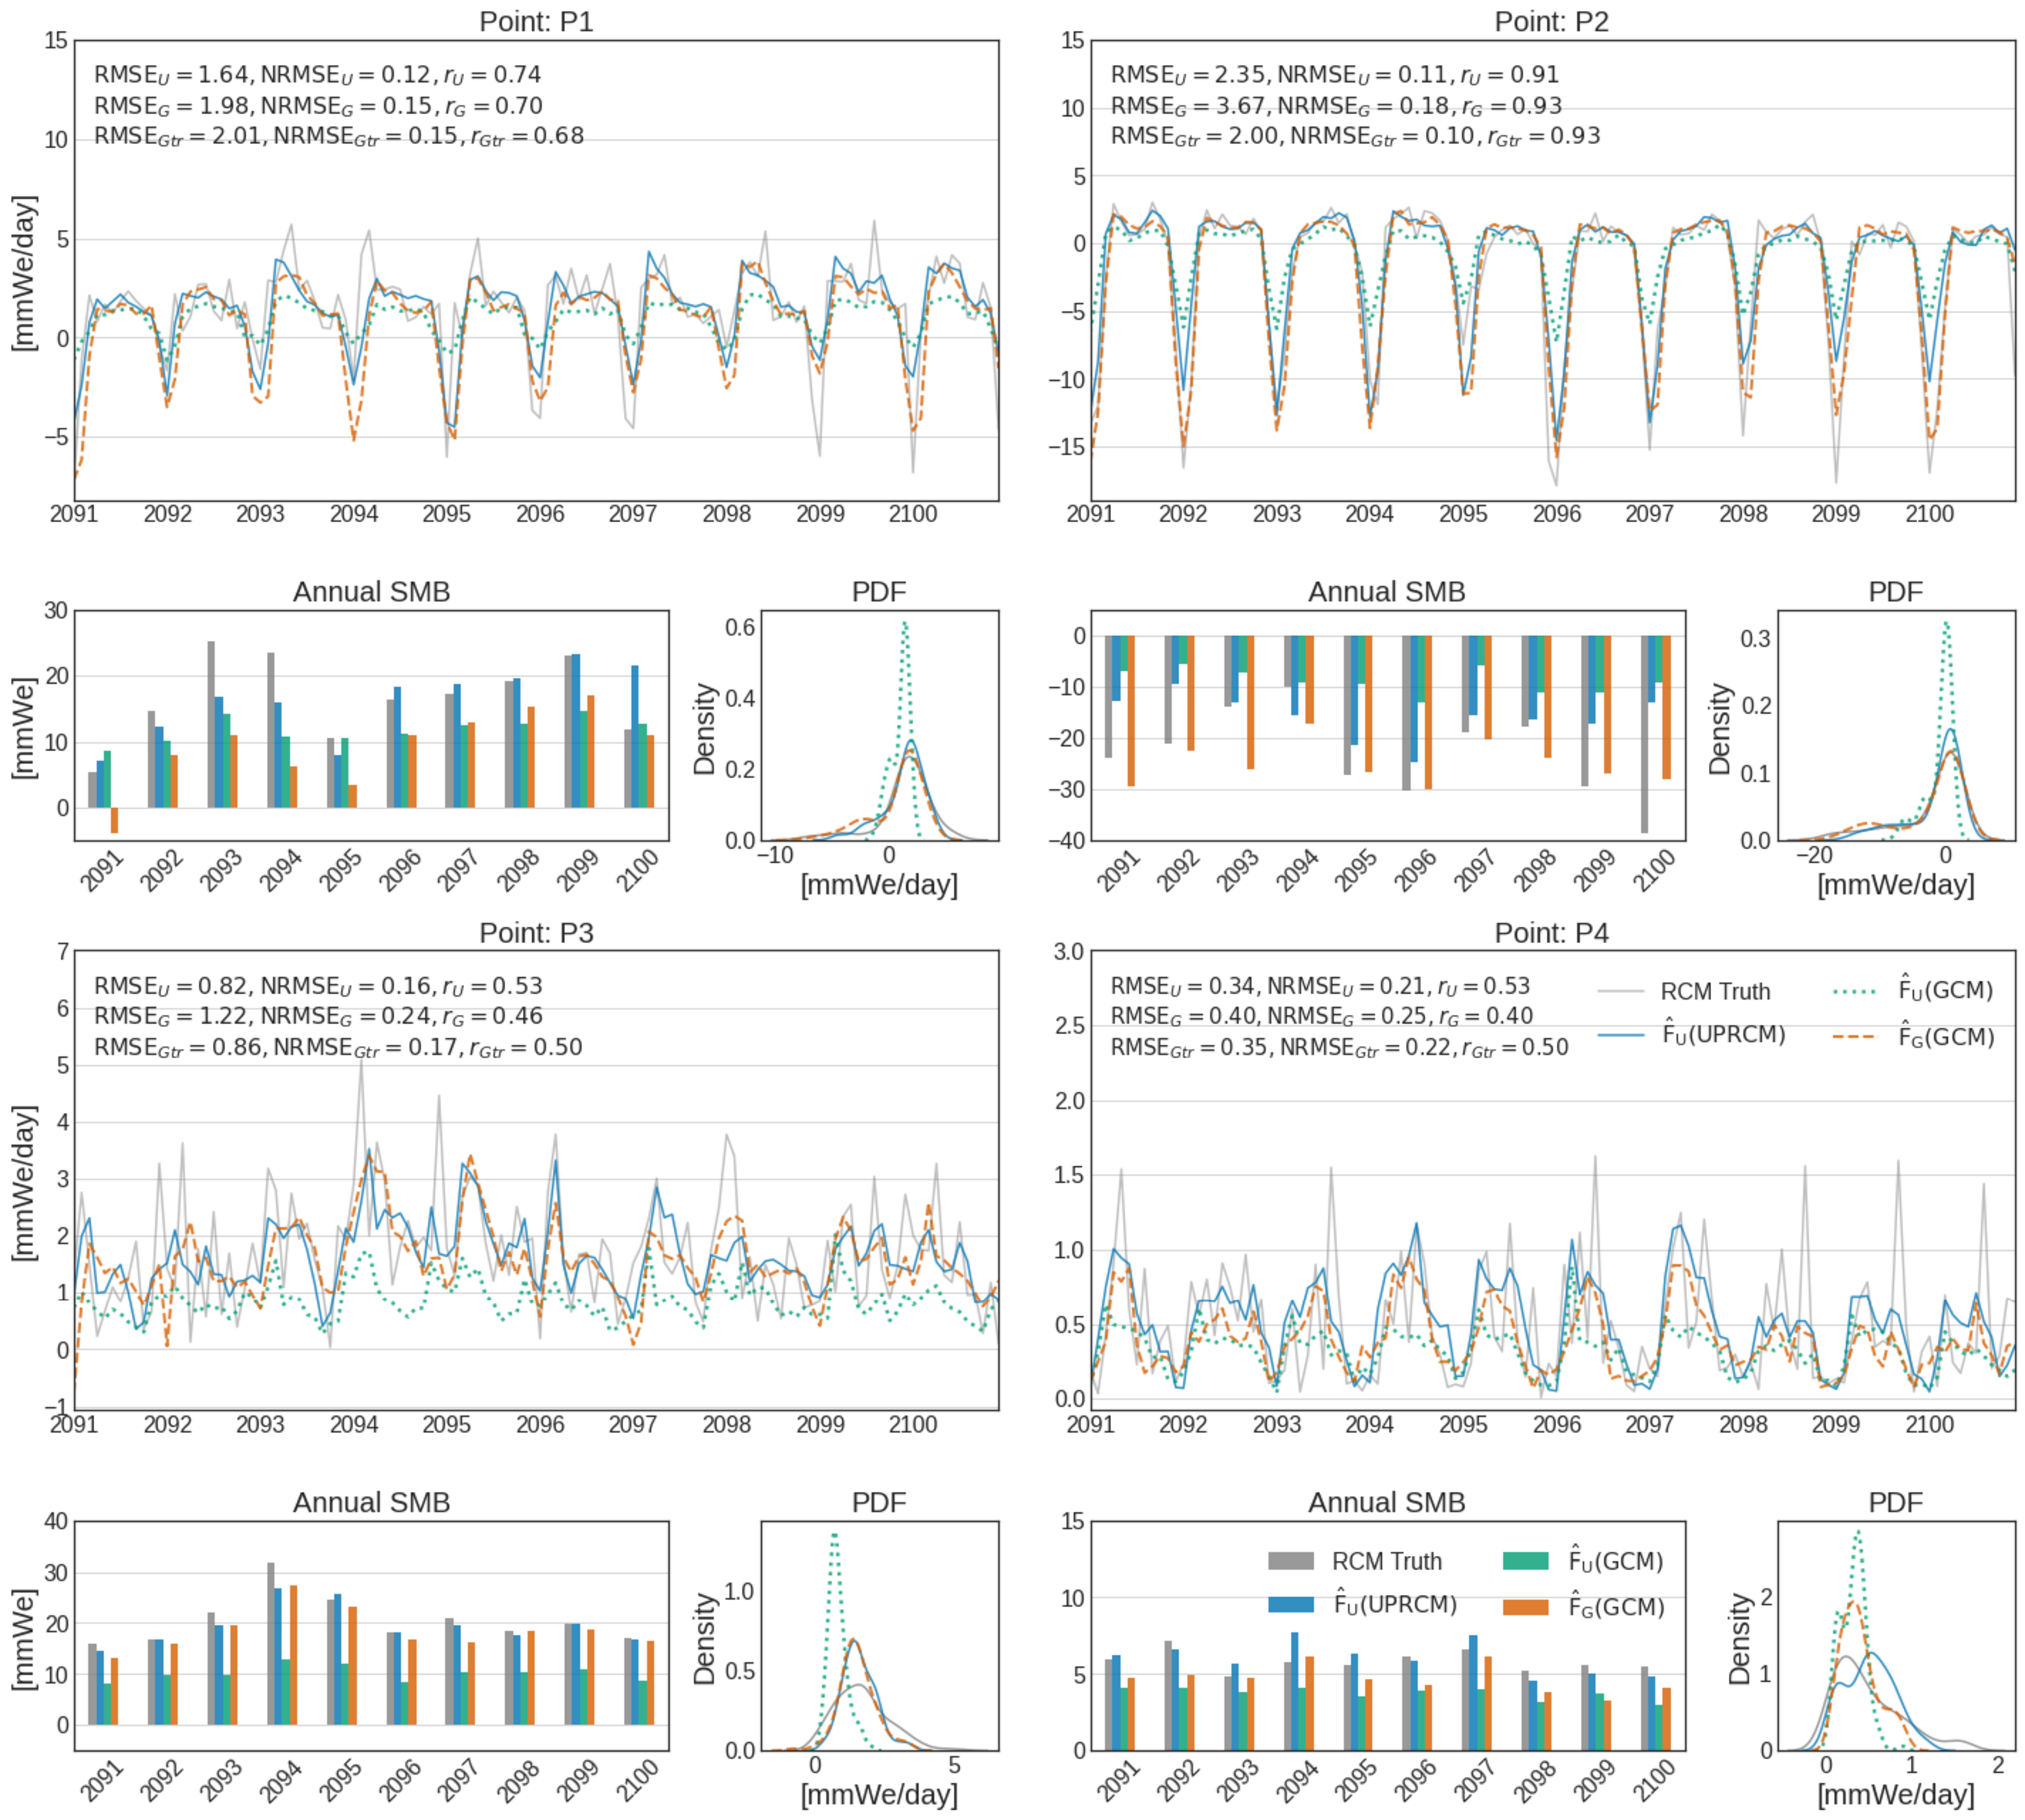
\includegraphics[width=\textwidth]{doc/Thesis-latex/images/results/timeseries_RCM_GCM.pdf}
            \caption[]%
            {{\small }}  
          \label{fig:timeseries-GCM-UPRCM}
        \end{subfigure}
        \hfill
        \caption[]
        {\small SMB predictions of RCM-emulators $\mathrm{\hat{F}_{U}(UPRCM)}$ (blue line), $\mathrm{\hat{F}_{U}(GCM)}$ (dotted green) and $\mathrm{\mathrm{\hat{F}_{G}(GCM)}}$ (dashed orange) compared to RCM truth (grey line) over test period (2090-2100). 
        (b) Time-series, daily probability density functions (PDF), and bar-plots of annual sums of SMB predictions for four different geographical points (a) in target domain $\mathcal{E}$.
        Legend: Pearson correlation coefficient ($\mathrm{r}$), RMSE ($\mathrm{RMSE}$), and normalized RMSE ($\mathrm{NRMSE}$) between the time series of emulated and true SMB. For these metrics $U$ = $\mathrm{\hat{F}_{U}(UPRCM)}$, $G$ = $\mathrm{\hat{F}_{U}(GCM)}$ and $Gtr$ = $\mathrm{\hat{F}_{G}(GCM)}$.} 
        \label{fig:points-timeseries-GCM-UPRCM}
    \end{figure}

\section{Evaluation metrics}
We used three traditional machine learning metrics as described in \autoref{subsec:evaluation-metrics} to evaluate the overall performance of emulators   $\mathrm{\hat{F}_{U}}$ and $\mathrm{\hat{F}_{G}}$ in reproducing the RCM truth. Results can be seen in \autoref{fig:evaluation-GCM-RCM}. We were particularly interested in seeing how the evaluation metrics differed for regions with high magnitudes of SMB (i.e., high precipitation levels), such as the tip and west coast of the Antarctic Peninsula, and dryer regions, such as the east coast and mainland. 

\textbf{Pearson correlation coefficient}: As seen in the box-plot of the correlation values, on average, SMB predictions from $\mathrm{\hat{F}_{U}(UPRCM)}$ and $\mathrm{\hat{F}_{G}(GCM)}$ have higher correlation values to the RCM truth than $\mathrm{\hat{F}_{U}(GCM)}$. This is especially flagrant on the tip and west coast of the Antarctic Peninsula, where $\mathrm{\hat{F}_{U}(UPRCM)}$ and $\mathrm{\hat{F}_{G}(GCM)}$ show the highest correlation to the target, with values close to 1. The east coast of the Peninsula has the lowest correlation for all models but especially for $\mathrm{\hat{F}_{U}(GCM)}$. We suspect this is because the model's predictions underestimate the temporal SMB patterns of dry regions. 

 \textbf{Wasserstein distance and RMSE}: $\mathrm{\hat{F}_{U}(GCM)}$ has the highest Wasserstein distance and RMSE values, which indicates that the density probability functions of its emulated SMB series are farther from the RCM truth. The Antarctic Peninsula has especially high differences in distributions, with outliers with values up to 10 for the Wasserstein distance and 14 for RMSE. This hints that the $\mathrm{\hat{F}_{U}(GCM)}$ emulator is not able to predict high SMB magnitudes when given GCM inputs while trained on UPRCM.   


Overall, we see that according to these evaluation metrics, $\mathrm{\hat{F}_{U}(UPRCM)}$ and $\mathrm{\hat{F}_{G}(GCM)}$ perform very similarly and are consistently better than $\mathrm{\hat{F}_{U}(GCM)}$. While temporal patterns and seasonality are best reconstructed in regions of high precipitation, such as the tip and west coast of the Antarctic Peninsula, the emulators' predictions tend to underestimate extreme (high and low) values. This is especially visible for $\mathrm{\hat{F}_{U}(GCM)}$ and in dry regions, such as the inland and east Peninsula. 


% evaluation metrics
\begin{figure}[!ht]
  \centering
  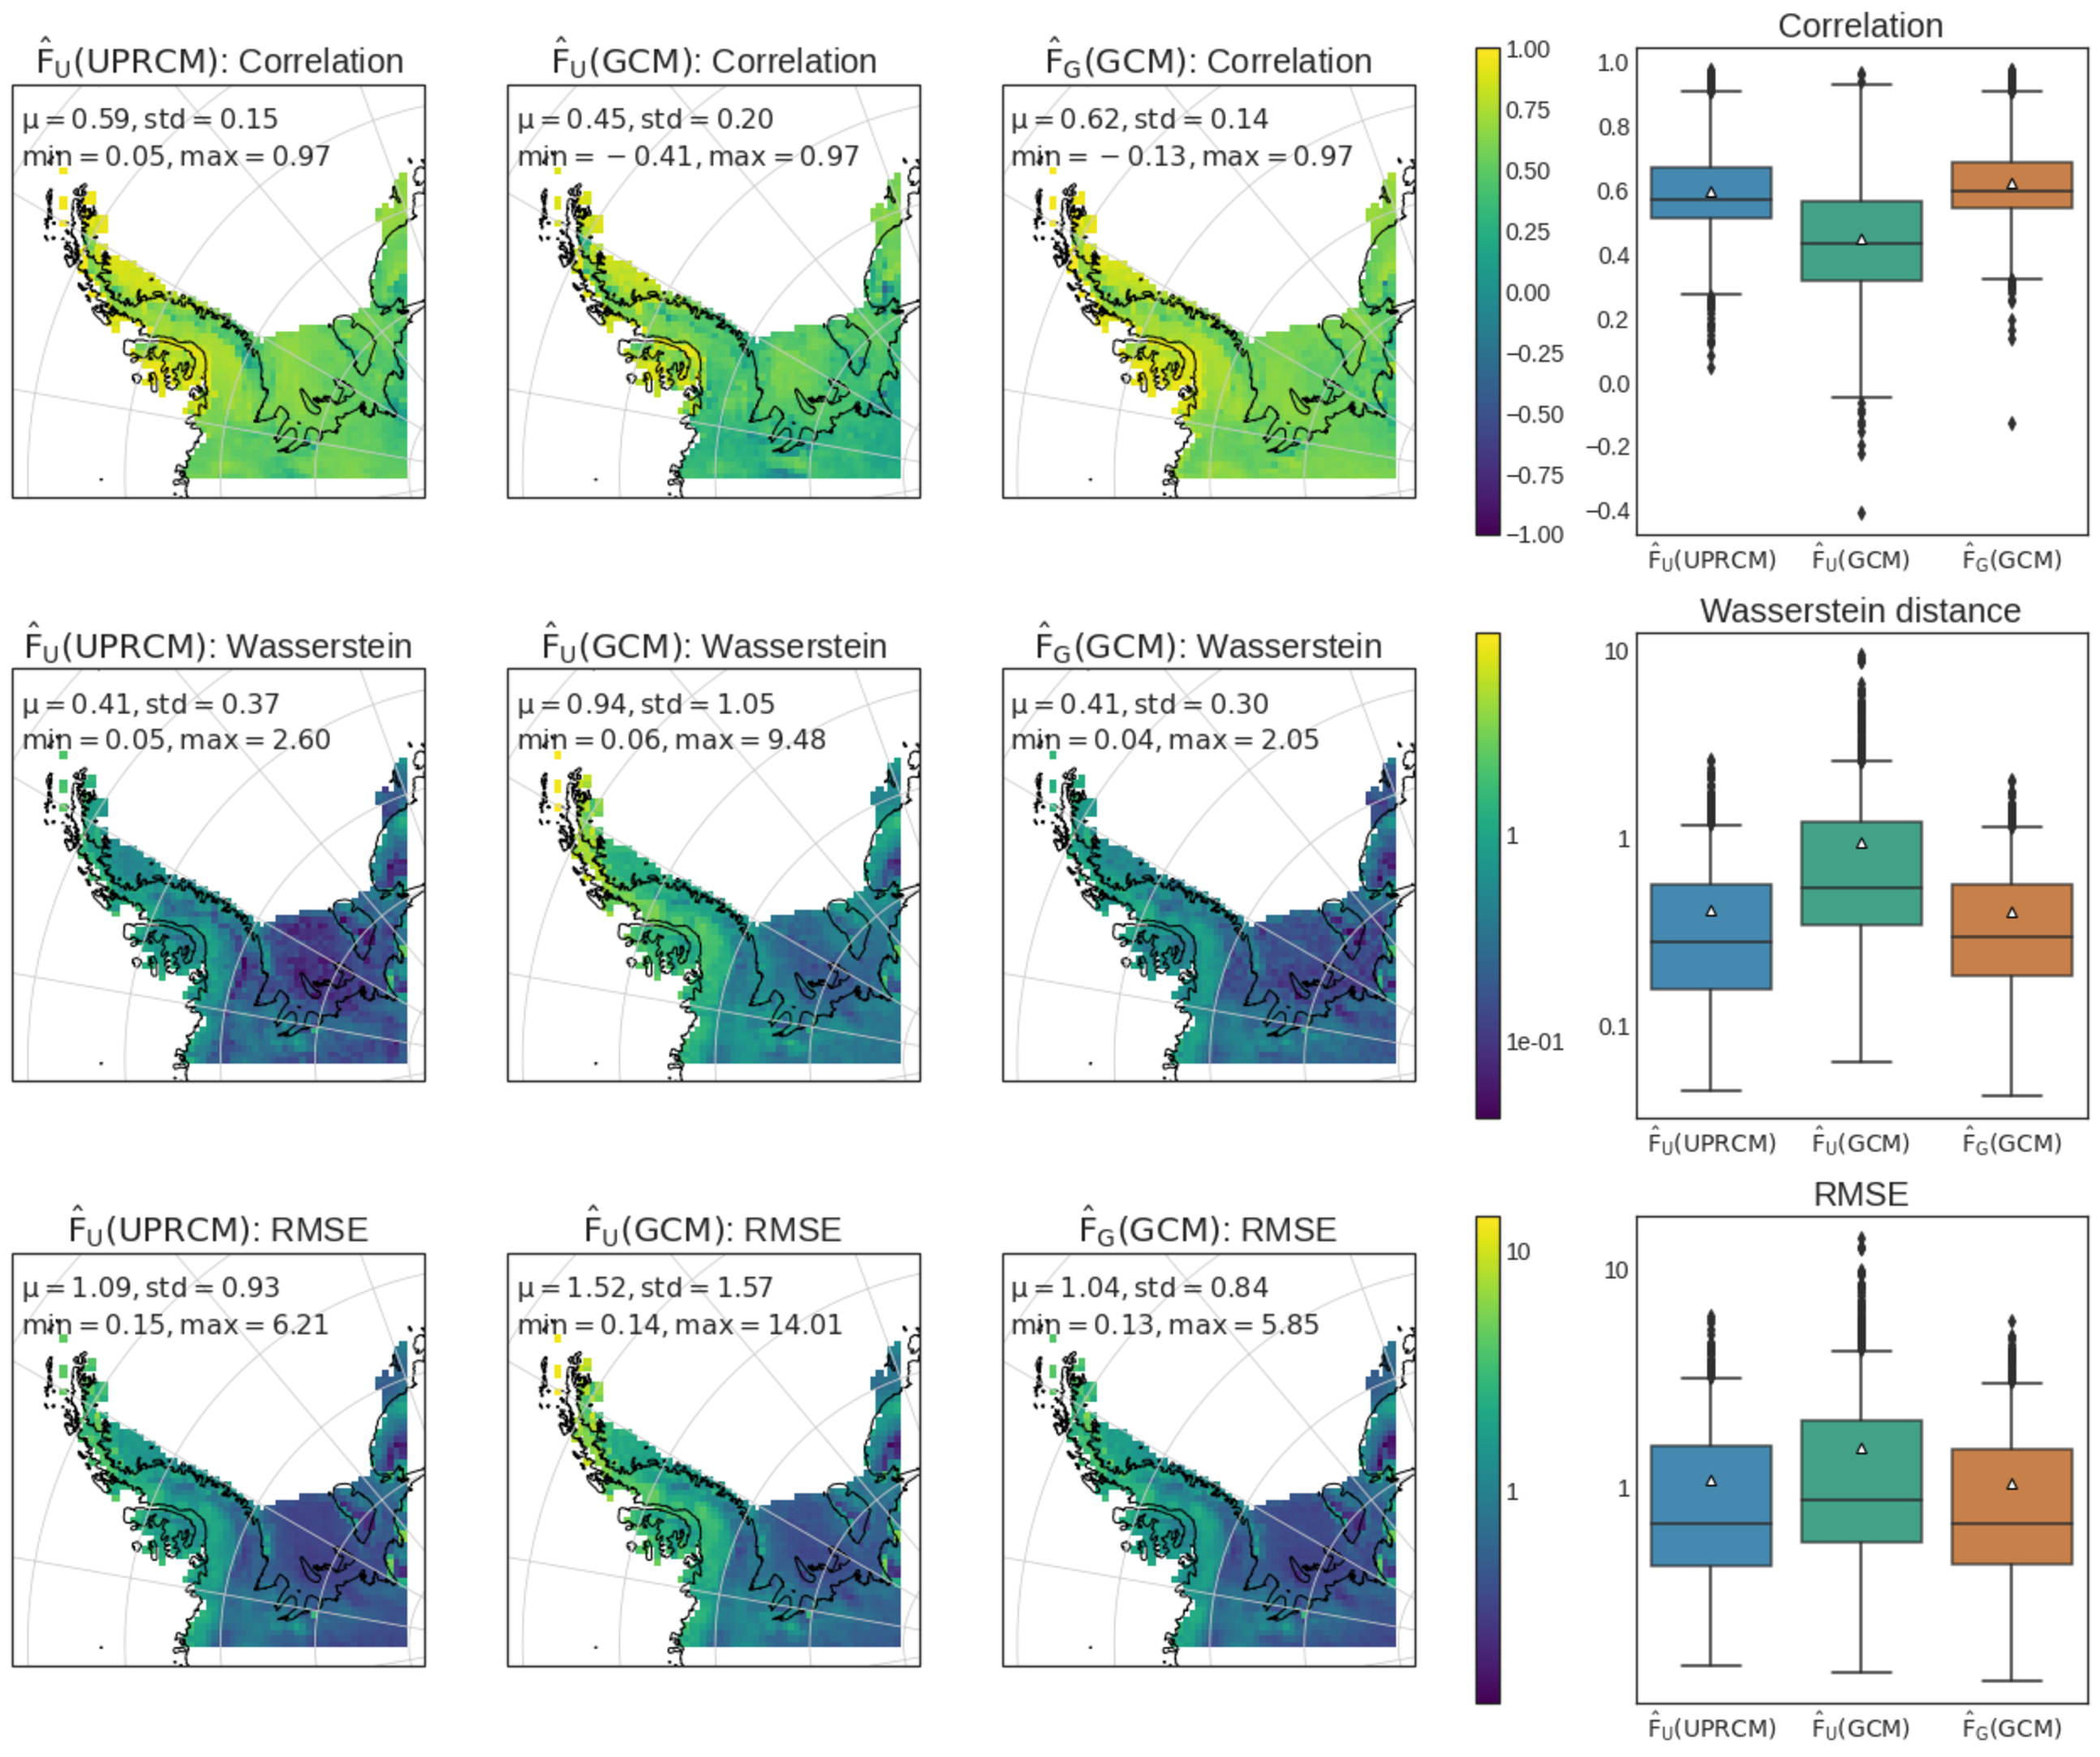
\includegraphics[width=\columnwidth]{doc/Thesis-latex/images/results/metrics_RCM_GCM.pdf}
  \caption []{\small Evaluation of predictions from RCM-emulators $\mathrm{\hat{F}_{U}(UPRCM)}$,  $\mathrm{\hat{F}_{U}(GCM)}$ and $\mathrm{\hat{F}_{G}(GCM)}$ over target domain $\mathcal{E}$ and test period (2090-2100). At each position, $p \in\mathcal{E}$, the time series of the true SMB are compared to predicted SMB values. Right: box-plot of evaluation metrics, from lower to upper quartile, with a line at the median and triangle at the mean. From top to bottom: Pearson correlation coefficient, Wasserstein distance, and RMSE as in \autoref{subsubsec:rmse}. Legend: spatial mean ($\operatorname{\mu}$), standard deviation ($\operatorname{std}$), minimum ($\min$) and maximum ($\max$) of metrics over $\mathcal{E}$.}
  \vspace{-3mm}
  \label{fig:evaluation-GCM-RCM}
\end{figure}

\section{Bias between UPRCM and GCM variables}\label{sec:res-bias-RCM-GCM}
To assess the bias and inconsistencies between the large-scale (low-resolution) and local-scale (high-resolution) atmospheric variables, we calculated the temporal and spatial correlation between UPRCM and GCM features (\autoref{eq:temporal-corr} and~\ref{eq:spatial-corr}). Results are illustrated in~\autoref{fig:corr-GCM-RCM}. 

\subsubsection{Temporal correlation}
For most atmospheric variables, the time series of URPCM and GCM features are highly positively correlated, with values very close to one (\autoref{fig:temp-corr-GCM-UPRCM}). However, the two wind variables (EW, NW) show inconsistencies between large and local-scale time series over the mainland and the Antarctic Peninsula, with minimal correlation values reaching 0.2. This suggests that, except for the winds, there is almost no inconsistency in the seasonal patterns between regional high-resolution and global low-resolution variables.

\subsubsection{Spatial correlation}
 Atmospheric variables like temperature, specific humidity, radiation, and precipitation show significant changes in spatial correlation between UPRCM and GCM features (\autoref{fig:spatial-corr-GCM-UPRCM}). The most flagrant variables are shortwave downward radiation (SWD) and precipitation (PR). SWD has an annual spatial correlation pattern strongly oscillating between approximately 0.2 in winter and 0.8 in summer. On the other hand, PR has a very poor spatial correlation over the whole test period, with a maximum of only 0.4. Looking at some individual months of those variables, we see that for SWD, the spatial correlation is low between UPRCM and GCM maps during winter because the GCM predicts higher radiation values in the mainland of Antarctica than UPRCM (\autoref{fig:spatial-corr-GCM-RCM-ex}). However, because there is very little radiation, spatial correlation is high for the summer months. For precipitation, the spatial patterns in the UPRCM and GCM are very different, with the UPRCM being much more precise in its predictions. For example, for November 2093, the UPRCM shows a local high-intensity precipitation event on the tip of the Antarctic Peninsula, while the GCM predicts a more vague pattern of lower intensity over the water in the west. We also notice a streak pattern on the left boundary of the RCM for all variables, but this is a known problem as the boundaries of climate models are usually imprecise. 

Overall, we found problems in consistency between large GCM and local-scale RCM variables. As mentioned in \autoref{subsec:perfect-model}, these inconsistencies might confuse an RCM-emulator, and this might justify the need for the perfect model framework for training a model. 


\begin{figure}[!h]
        \centering
        \begin{subfigure}[b]{\columnwidth}
            \centering 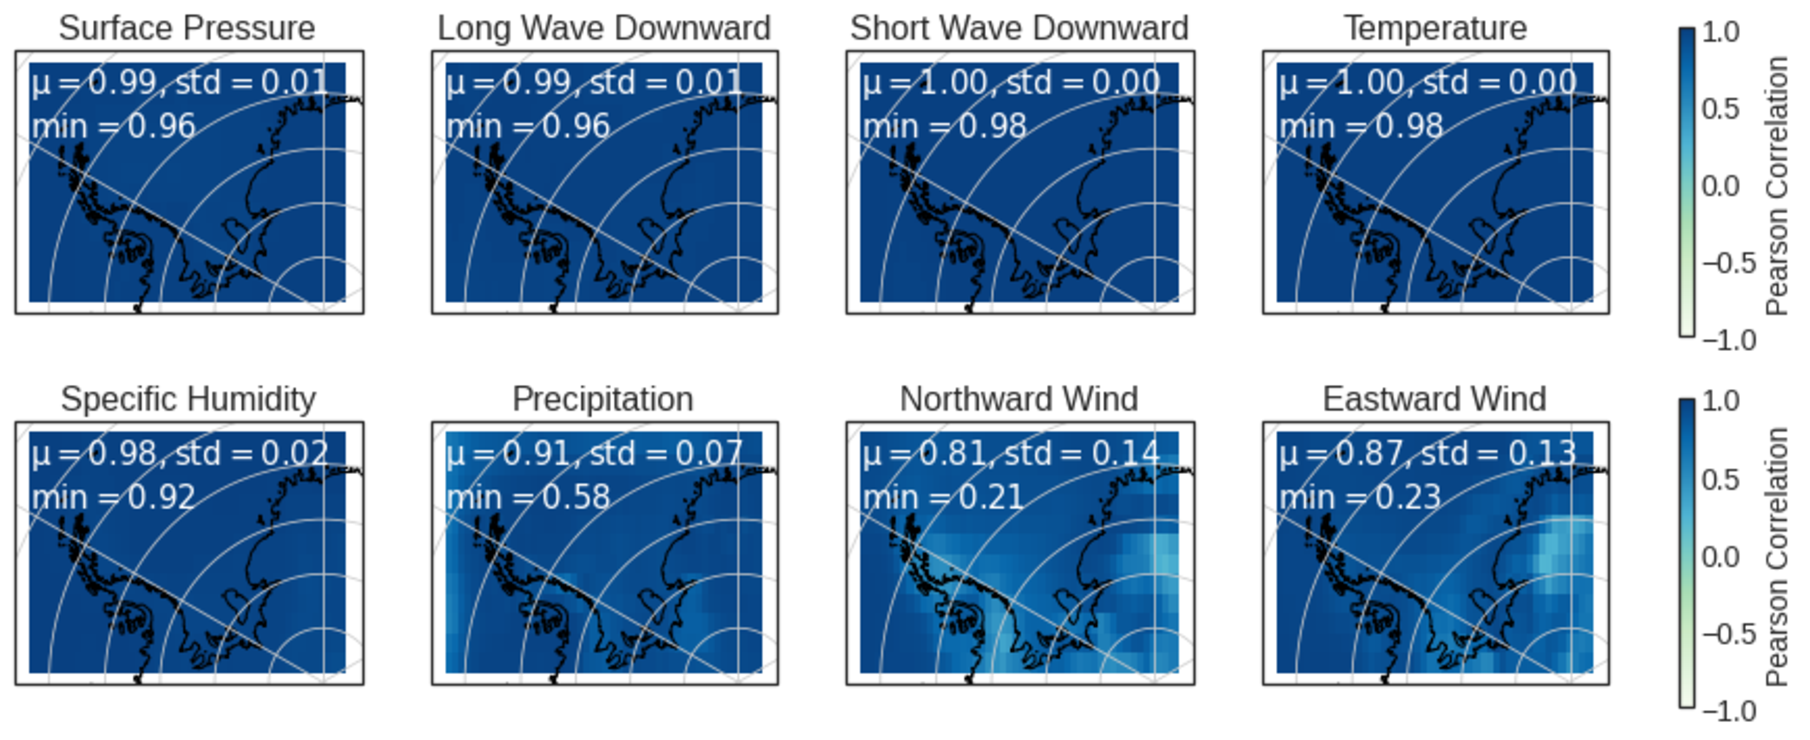
\includegraphics[width=\textwidth]{doc/Thesis-latex/images/results/temporalCorr_RCM_GCM.pdf}
            \caption[]%
            {{\small Temporal correlation}}    
          \label{fig:temp-corr-GCM-UPRCM}
        \end{subfigure}
        \hfill
            \begin{subfigure}[b]{\columnwidth}
            \centering 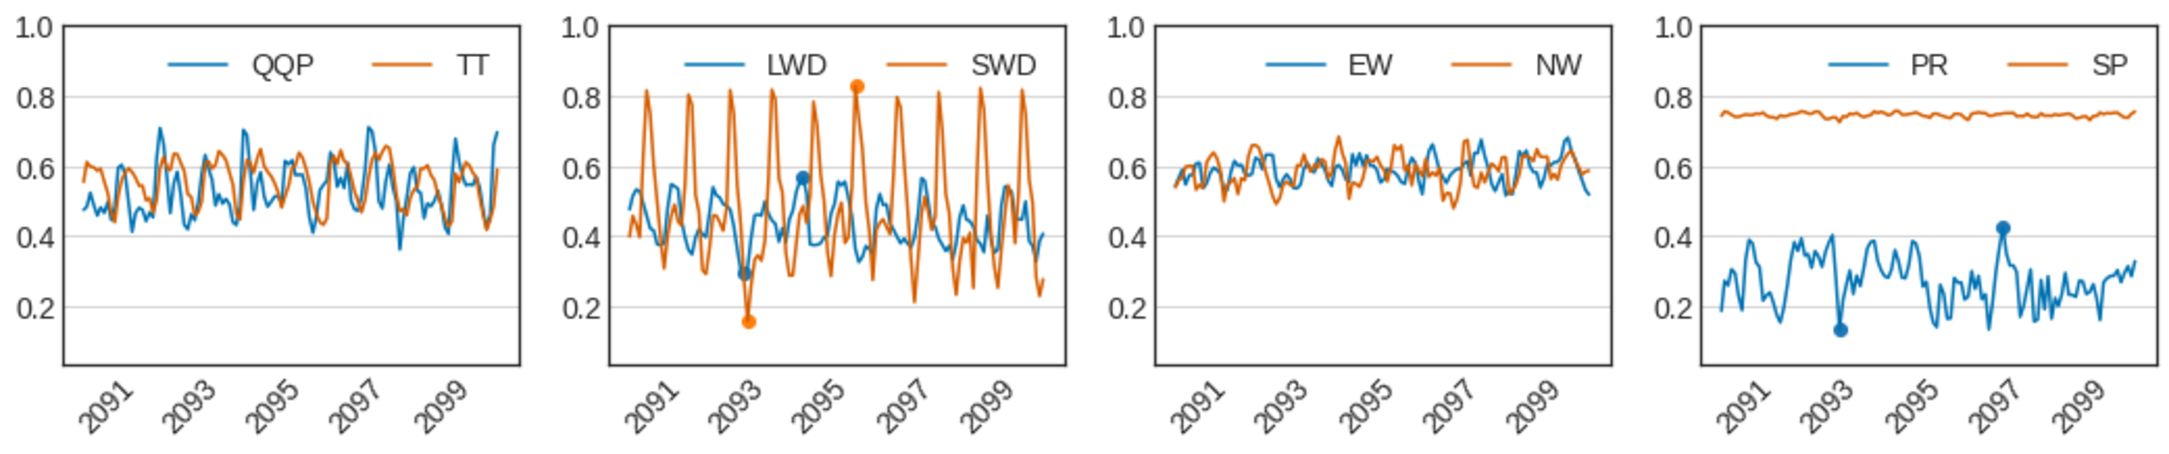
\includegraphics[width=\textwidth]{doc/Thesis-latex/images/results/spatialCorr_TS_RCM_GCM.pdf}
            \caption[]%
            {{\small Spatial correlation}}    
          \label{fig:spatial-corr-GCM-UPRCM}
        \end{subfigure}
        \hfill
        \begin{subfigure}[b]{\columnwidth}  
            \centering 
            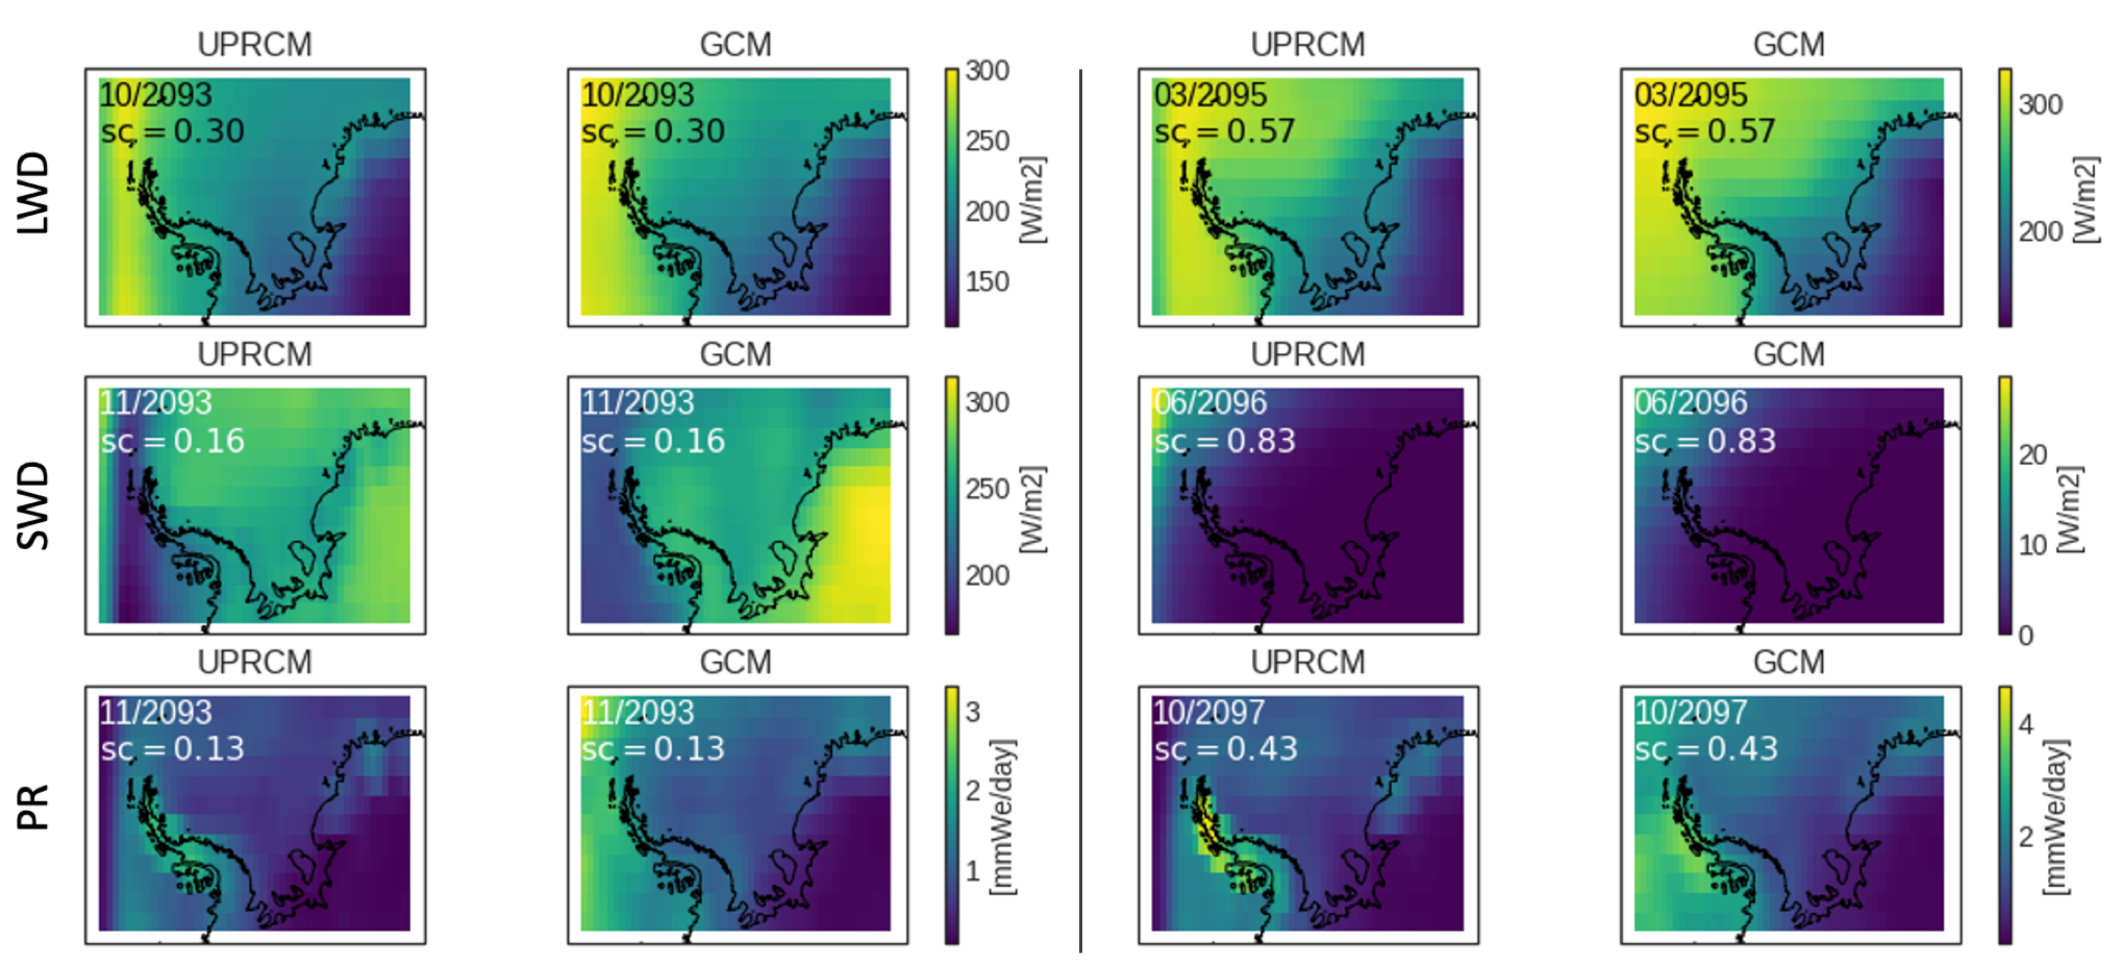
\includegraphics[width=\textwidth]{doc/Thesis-latex/images/results/spatialCorr_RCM_GCM.pdf}
            \caption[]%
            {{\small Spatial patterns for LWD, SWD and PR for example months}} \label{fig:spatial-corr-GCM-RCM-ex}
        \end{subfigure}
        \hfill
        \caption[]
        {\small Temporal (a) and spatial (b, c) correlation between UPRCM and GCM variables given as input to RCM-emulator over target domain $\mathcal{E}$ and test period (2090-2100). (a) Pearson correlation coefficient between UPRCM and GCM time series for each point $p$ in $\mathcal{E}$. Legend: mean ($\mu$), standard deviation ($\operatorname{std}$) and minimum ($\min$) of correlation values over $\mathcal{E}$. (b) Spatial correlation between UPRCM and GCM variable maps over $\mathcal{E}$ at each time step. (c) Example of months with lowest (left) and highest (right) spatial correlation ($\operatorname{sc}$) between UPRCM and GCM for long/short-wave downward radiation (LWD/SWD) and precipitation (PR). Chosen months are illustrated with dots on the time series in (b).} 
        \label{fig:corr-GCM-RCM}
    \end{figure}


\section{Computational efficiency}\label{sec:computational-efficiency}
Using early stopping as described in~\autoref{subsec:training}, RCM-emulators $\hat{F}_U$ and $\hat{F}_G$ trained for 31 and 40 epochs before stopping. Training took approximately 4 minutes, with roughly 6 seconds per epoch. A GPU is no longer needed once the model is trained, and making predictions on test data takes 15 seconds on a CPU, which is nearly instantaneous. This computational time is significantly smaller than running an RCM simulation which can take multiple weeks to calculate on a super-computer. Note that our computational time does not include data preparation for the RCM-emulator. But if the data is readily obtainable and a correct data processing pipeline is in place, selecting the target region and creating the UPRCM takes only a few hours on a CPU.



\chapter{Discussion}
%%%%%%%%%%%%%%%%%%%%

\section{Extending an emulator of near-surface temperature to SMB}\label{sec:extension-doury}

In this thesis, we extended the machine learning model that emulated near-surface temperature over the south of France, proposed by Doury et al.~\cite{Doury} to emulate SMB over the Antarctic Peninsula. In doing so, we faced different challenges because SMB is notoriously difficult to observe and represent compared to temperature~\cite{Lenaerts2019}. 


Since temperature is a variable present in both the GCM and RCM, it was amidst the low-resolution features given as input to the temperature emulator from Doury et al.~\cite{Doury}. In our case, SMB was only available in the RCM. Thus, our emulator could reconstruct a high-resolution image of SMB given only a limited number of other atmospheric variables that did not include a low-resolution image of SMB. This might explain why the SMB patterns of some regions in the Antarctic Peninsula, especially those with less seasonal patterns (e.g., P3 in \autoref{fig:points-timeseries-GCM-UPRCM}), might be more challenging for the model to reconstruct. We rely on the assumption that our model has a clear physical relationship to learn between our eight large-scale atmospheric variables and local-scale SMB, but this might not be true for all points in the Peninsula. There might be regions where the factors influencing SMB are more complex than the variables we have and where the model might benefit from additional information, such as other large-scale atmospheric variables, ice sheet topography, or past SMB patterns. This could be explored in further work.


For their temperature emulator, Doury et al. had seven atmospheric variables at different pressure levels at their disposition, resulting in 19 input features. Unfortunately, because our chosen dataset had only eight surface-level variables, we could only train our model on eight features. Doury et al. found that while more inputs in their model seemed to improve the quality of the emulated series, having a "cheaper" model with fewer inputs showed satisfying results and could be regarded as a suitable option~\cite{Doury}. While we ideally wished to have more variables to help our emulator reconstruct regional SMB over the Antarctic Peninsula, having a "cheaper" model at least gave a higher computational gain (4 minutes of training compared to 2 hours in~\cite{Doury}).  


Ice sheet SMB varies highly across multiple space and time scales~\cite{Lenaerts2019}. For example, as was discussed in \autoref{sec:res-time-series}, on the Antarctic Peninsula, while some regions have high seasonal amplitude changes in SMB, others have (almost) none. This was not the case for the near-surface temperature emulated in~\cite{Doury}, where, even though their target domain (southern France with the Pyrenees) covered different climates, its temperature fluctuated in approximately the same annual amplitude range for all points in their domain. Therefore, opposite to the model developed by Doury et al., our model had to acclimate different scales in SMB values over the Peninsula. For this, we used a normalized RMSE loss and attention mechanisms, but our emulator still better reconstructs regions with high seasonal change. The results hint that NRMSE and attention might not be enough to account for different scales in target values and should be adapted in further work. 


\section{Necessity of the perfect model framework}\label{sec:disc-perfect-model}

As outlined in \autoref{subsec:training}, we trained two RCM-emulators separately; one followed the perfect model framework ($\mathrm{\hat{F}_{U}}$) and another directly trained with large-scale GCM data ($\mathrm{\hat{F}_{G}}$). 


Doury et al. state that the perfect model framework is necessary to learn the RCM downscaling function without any interfering biases between the GCM and RCM. However, to be useful, the RCM-emulator should give accurate reconstructions of SMB when given large-scale GCM variables as input. Otherwise, the model would not be valuable if it needs upscaled RCM features to make predictions. Nevertheless, while the predictions of $\mathrm{\hat{F}_{U}(GCM)}$ follow the correct temporal patterns of the RCM truth, they consistently underestimate the truth and produce a toned-down version of the true SMB time series. We suspect this is because, under the perfect model framework, the emulator cannot learn GCM-RCM inconsistencies during its training. Consequently, when the model is given GCM inputs while trained on UPRCM, inconsistencies are preserved and appear in the local reconstructions. This problem was also found by Doury et al. for their temperature emulator~\cite{Doury}. 


As shown in \autoref{sec:res-bias-RCM-GCM}, we find significant bias and inconsistencies between RCM and GCM variables. For example, the two wind variables showed high temporal discrepancies between large and local-scale simulations. This might happen if there is an offset in the RCM time series compared to the GCM or if the patterns are completely different. Furthermore, we also found spatial inconsistencies for most atmospheric variables, especially for precipitation and downward radiation. Some of this bias might exist for problematic reasons, such as inconsistent forcings or boundary conditions when RCM simulations are computed. We suspect this might be the reason for the streaks visible on the left boundary of RCM images in~\autoref{fig:spatial-corr-GCM-RCM-ex}. However, we assume that the rest of the inconsistencies exist because the RCM adjusts the low-resolution simulation for valid reasons i.e., for a more fine-scaled simulation of the physical processes~\cite{Doury, S_rland_2018, Vasubandhu2007, Noguer1998, Laprise2008ChallengingST}. 


 We trained the second emulator $\mathrm{\hat{F}_{G}}$ directly with large-scale GCM inputs to see whether it could account for the RCM-GCM inconsistencies. $\mathrm{\hat{F}_{G}(GCM)}$ misses some precision compared to $\mathrm{\hat{F}_{U}(UPRCM)}$ in emulating SMB patterns for regions with minor SMB variations (e.g. P4 in~\autoref{fig:points-timeseries-GCM-UPRCM}, SMB smaller than 1.5 \si{mmWe/day}). But for the other points, $\mathrm{\hat{F}_{G}(GCM)}$ comes very close to the RCM truth. It is also performing exceedingly well in terms of predicting annual SMB values and is consistently better than $\mathrm{\hat{F}_{U}(GCM)}$. 


Under the assumption that most of the GCM-RCM inconsistencies exist for valid reasons, it seems like the perfect model framework may not be necessary to train our RCM-emulator. When trained with low-resolution GCM data, the model can predict SMB values close to the truth, as if it learned the underlying RCM-GCM inconsistencies and dynamics.   



\section{Usability of the RCM-emulator}\label{sec:utility-emulators}
For our RCM-emulator to be practical, it has to be faster and easier to use than computing an RCM simulation. We showed in \autoref{sec:computational-efficiency} that training the emulator and making predictions is very fast, with predictions made nearly instantaneously and training in 4 minutes. The primary time bottle-neck for a user might be getting the correct data and pre-processing it to fit the desired training setting. In the following, we will explore how easy the model is to use. 

\subsubsection{Transparency}
Neural networks have a reputation for being a black box algorithm with a decision process that is hard to understand. This is not different in our case. Because we give all available variables to our model without making any uphill feature selection, it would be interesting to know which physical features carry the most weight in the model's decision. Even though there are new ways to try to open the black box~\cite{Guidotti, Shwartz2017}, it remains a challenging problem for which we, unfortunately, did not have more time to explore. While traditionally, computing an RCM allows the user to have complete control over things such as variables, forcings, and boundary conditions, using a machine learning emulator offers less transparency.

\subsubsection{Randomness and reproducibility}
Training a neural network while relying on a GPU creates several sources of randomness~\cite{Zhuang2021, Reproducibility}. To make our model reproducible, we used a fixed seed, and in this setting, our model always gives the same predictions. Nevertheless, another seed might provide very different results, so to reproduce our results, one must be careful to use the same random settings. To assess the robustness of our RCM-emulator, one could run it several times using different seeds and observe the average results. Due to time constraints, this was omitted. 

\subsubsection{Specificity of the RCM-emulator}
One limitation of our RCM-emulator is that it focused only on reconstructing one target domain, the Antarctic Peninsula. If one wanted to expand it to other areas, one would have to re-train the model on data of this specific region. We suspect that applying our emulator elsewhere would not work otherwise, as it would be faced with images very different from its training. However, we believe that because the emulator works well for the Peninsula, an area that shows high variability in SMB patterns, it will perform just as well for other domains of Antarctica once it has been correctly trained. In further work, we could also envision training the emulator on a more extensive dataset containing several regions of Antarctica or using techniques like transfer learning and domain adaptation so that the model can reproduce new areas.  

Furthermore, if one wanted to extend the emulator to other climate model simulations, one would also need to re-train it for those climate models. One exception might be if they are similar to ACCESS 1.3 and MAR(ACCESS1.3). For example, one could try making predictions with our emulator on another future RCP simulation of MAR(ACCESS1.3), such as RCP4.5.  

\subsubsection{Data availability}
The ACCESS 1.3 GCM data is openly available to the public on the Australian NCI \href{https://esgf.nci.org.au/search/esgf-nci/}{website}~\cite{NCI}. We had to ask for the MAR(ACCESS1.3) RCM data from the Geo-science Institute of the University of Grenoble. Therefore, while acquiring GCM data is easy, getting access to RCM simulations might be more challenging for a lambda user.

\subsubsection{Code availability}
The trained RCM-emulators, notebooks, and python scripts for pre-processing and machine learning are available on our \href{https://github.com/marvande/master-thesis}{GitHub} repository~\cite{GitHub}. For any questions or additional information about the code, email: \href{mailto:marijn.vandermeer@bluewin.ch}{marijn.vandermeer@bluewin.ch}. 


%%%%%%%%%%%%%%%%%%%%
\chapter{Conclusion}
%%%%%%%%%%%%%%%%%%%%

In this thesis, we built a machine learning model called the RCM-emulator that reconstructs local-scale surface mass balance (SMB) values over the Antarctic Peninsula by learning the downscaling function of a regional climate model (RCM). This means that our model, when given large-scale (low-resolution) atmospheric variables from a global climate model (GCM), can reconstruct a local-scale (high-resolution) image of SMB from an RCM. Compared to running an RCM, the emulator is designed to be computationally faster.   

Our model is an extension of a U-Net model proposed by Doury et al. that emulated near-surface temperature over the south of France~\cite{Doury}. We extended their U-net by adding convolutional block attention mechanisms in the encoder of the U-Net and replaced traditional convolutional operations with depthwise-separable convolutions. Furthermore, to account for the different scales of SMB values across the Antarctic Peninsula, we used a normalized RMSE. 

For training our model, we proposed two frameworks. The first is a perfect model framework where the emulator received low-resolution inputs from the RCM upscaled to GCM resolution instead of the GCM. For this, we created large-scale features from RCM with interpolation (UPRCM). This setting was designed so that the model learned the downscaling function undisturbed by potential GCM-RCM inconsistencies and biases. In the second framework, we trained the model on large-scale features directly sourced from the GCM to evaluate whether it could make accurate predictions despite those inconsistencies. 

Training our model takes under four minutes on a GPU, and predictions are almost instantaneous, but data gathering and pre-processing can be time-consuming. However, our emulator is significantly faster than an RCM simulation, which can take several weeks on a supercomputer. 

We evaluated the first emulator, trained in the perfect model setting, on large-scale UPRCM features and, in a second step, directly with variables from the GCM. While the emulator evaluated on UPRCM features can almost perfectly reproduce the high-resolution SMB truth, predictions made with GCM features consistently underestimate it. This is not surprising as we find high spatial and temporal bias while exploring the consistency between GCM and RCM features. Because the perfect model framework does not allow the emulator to learn large-scale GCM-RCM inconsistencies, they are conserved when making predictions with GCM variables, leading to underestimation. 

The second emulator, trained directly on GCM features, could reproduce detailed high-resolution SMB maps. The model can make correct annual SMB predictions and reconstruct the temporal patterns of individual SMB time series and global spatial structures over the Antarctic Peninsula. Its only limitation is producing an accurate representation of points in dry climates where the normalized RMSE loss is insufficient to account for the small SMB values. In further work, one could focus on these climates to improve the emulator's predictions. Assuming that RCM-GCM inconsistencies exist for a valid reason and that we wish the emulator to account for them, our results indicate that a perfect model framework might not be needed and that our model can learn them.  


In conclusion, we built a machine learning RCM-emulator that can make fast and fine-scaled SMB reproductions over the Antarctic Peninsula from GCM data. Therefore, this emulator can be an interesting tool for providing low-cost local-scale information on the evolution of ice sheets during climate change. 

\cleardoublepage
\phantomsection
\addcontentsline{toc}{chapter}{Bibliography}
\printbibliography
% %%%%%%%%%%%%%%%%%%%%%%%%%%%%%%%%%%%%%%
% Appendices are optional
\appendix

\chapter{Data processing}

\section{Pre-processing of the GCM}\label{sec:preproc-GCM}

All pre-processing of the RCM and GCM data was done on \href{https://pangeo.io/about.html}{Pangeo}, a community platform for Big Data geoscience. First, we downloaded the ACCESS 1.3 GCM data from the Australian NCI \href{https://esgf.nci.org.au/search/esgf-nci/}{website}~\cite{NCI}. From their database, we chose the dataset with atmospheric variables (Amon) from the CMIP5 and r1i1p1 ensemble. As a time frame, we decided to use the historical and future RCP8.5 simulations, which are monthly mean aggregations of daily values. Now, the data can also be directly downloaded with the wget script on our \href{https://github.com/marvande/master-thesis}{GitHub}. 

From this GCM dataset, we chose the eight variables as seen in \autoref{tab:features}. To restrict the dataset size and because we were only interested in the region of Antarctica, we cut the data so that its latitude was between -40 and -90 $\si{\degree}$. Because the GCM is in latitude-longitude coordinates, but the RCM is in polar stereographic coordinates, we reprojected the GCM to the same projection system as the RCM. We did this by upsampling the RCM stereographic grid to cover approximately the same resolution as the GCM ($68 \times 206$ \si{km}) and then interpolated the GCM on that grid. We changed the units for the following variables to coincide with the RCM: 
\begin{itemize}
        \item Precipitation (PR): from \si{kg m^{-2}s^{-1}} to \si{mmWe/day}
        \item Surface pressure (SP): from \si{pa} to \si{hpa}
        \item Temperature (TT): from \si{K} to \si{C}
        \item Specific humidity (QQP): from \si{g/g} to \si{g/Kg}
    \end{itemize}
Finally, the GCM variables were smoothed by a $3\times3$ moving average filter to follow the same pre-processing procedure as for the temperature emulator in~\cite{Doury} (c.f. \autoref{subsec:perfect-model}). 


\section{Pre-processing of the RCM}\label{sec:preproc-RCM}
We acquired the MAR(ACCESS 1.3) RCM data from the Geoscience Institute of the University of Grenoble. Because ACCESS 1.3 was in monthly frequency, we did a monthly mean aggregation on the RCM. We also changed the spatial units from \si{km} to \si{m} to be in accordance with GCM units. 

Variables like the winds, temperature and specific humidity were initially provided for seven pressure levels (200, 500, 600, 700, 800, 850, and 925 \si{hpa}) while we needed surface-level values to coincide with the GCM. Each pressure level had NaN values where it intersected with the surface. So, for each point $p$ in the RCM domain, we took the last non-NaN value on the highest possible pressure level as the surface value (\autoref{fig:example-plevels}). Furthermore, RCM wind variables were given as x and y-components, while GCM winds were northward and eastward. Therefore RCM wind components needed to be reprojected to become north/eastward winds. First we calculated a grid that gave the latitude ($\mathrm{lat}$) and longitude ($\mathrm{lon}$) coordinates for each point $(i,j)\in X,Y \subset \mathcal{E}$ in the RCM polar stereographic grid $\mathcal{E}$. Then, for each point $(i,j)$ we applied Algorithm~\ref{alg:wind-components}.
    \begin{algorithm}
    \caption{Transformation of wind x/y-components into north/eastward}\label{alg:wind-components}
    \begin{algorithmic}[1]
    \State $\operatorname{GEddxx} = 90$
    \State $\Delta \phi = 90 - \operatorname{GEddxx}$
    \State $dr = \pi / 180$ 
    \For{$i,j \in X,Y$}
    \State $\phi \gets -1*dr*(\mathrm{lon}[i,j] + \Delta \phi)$
    \State $\mathrm{cphi} \gets cos(-\phi)$
    \State $\mathrm{sphi} \gets sin(-\phi)$
    \State  $\mathrm{windEast}[i, j] \gets \mathrm{cphi} * \mathrm{windX}[i, j] - \mathrm{sphi} * \mathrm{windY}[i,j]$ \Comment{Eastward wind component}
    \State $\mathrm{windNorth}[i, j] \gets  \mathrm{sphi} * \mathrm{windX}[i, j] + \mathrm{cphi} * \mathrm{windY}[i, j]$ \Comment{Northward wind component}
    \EndFor
    \end{algorithmic}[1]
    \end{algorithm}
\\ Finally, to create GCM-like low-resolution UPRCM features from the RCM, we reprojected the RCM on the GCM grid by interpolation. Then, we used the same moving average filter for the GCM to smooth the data (\autoref{fig:training-data-flow}). Finally, because there is no precipitation variable in the RCM, we created one by adding the snowfall and rainfall variables. 
    \begin{equation*}
        \mathrm{PR} = \mathrm{SF} + \mathrm{RF}
    \end{equation*}

\begin{figure}[!htb]
  \centering
  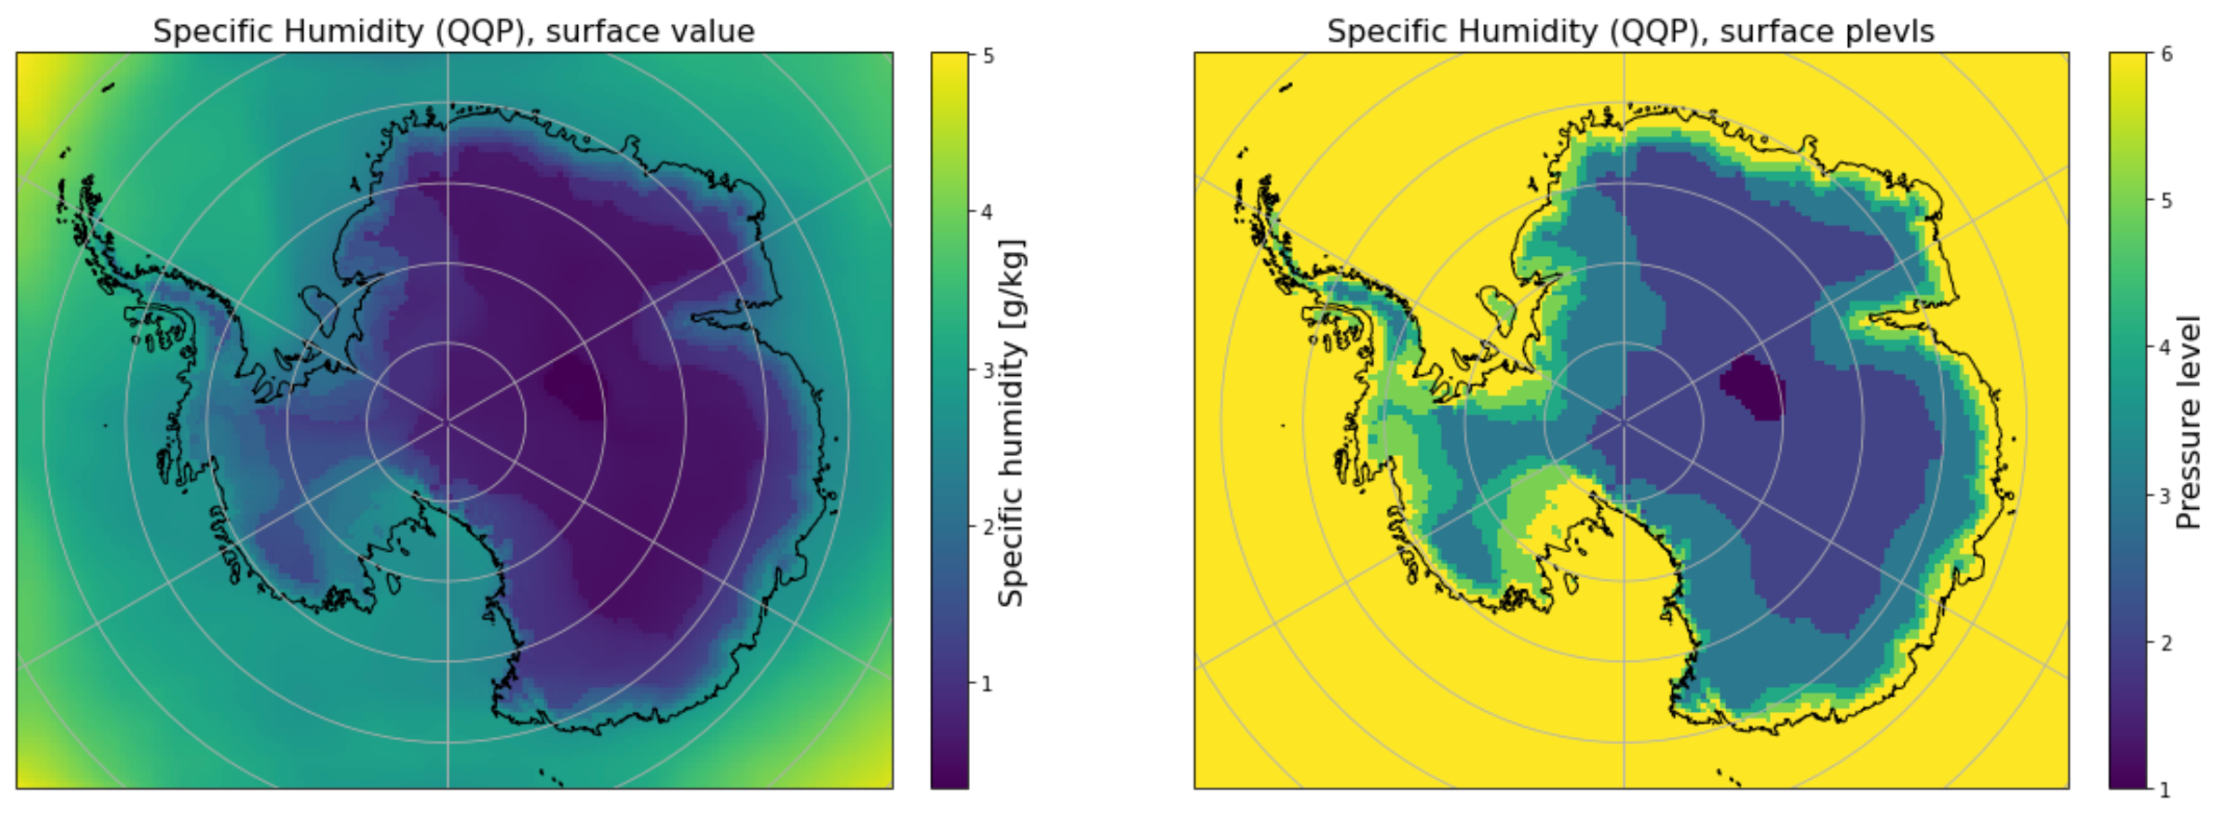
\includegraphics[width=\columnwidth]{doc/Thesis-latex/images/example-plevels.pdf}
  \caption []{\small Illustration of the process of changing the specific humidity (QQP) variable from values at different pressure levels to surface level values (left). Right: pressure at surface over Antarctica.}
  \vspace{-3mm}
  \label{fig:example-plevels}
\end{figure}

\begin{figure}[!htb]
  \centering
  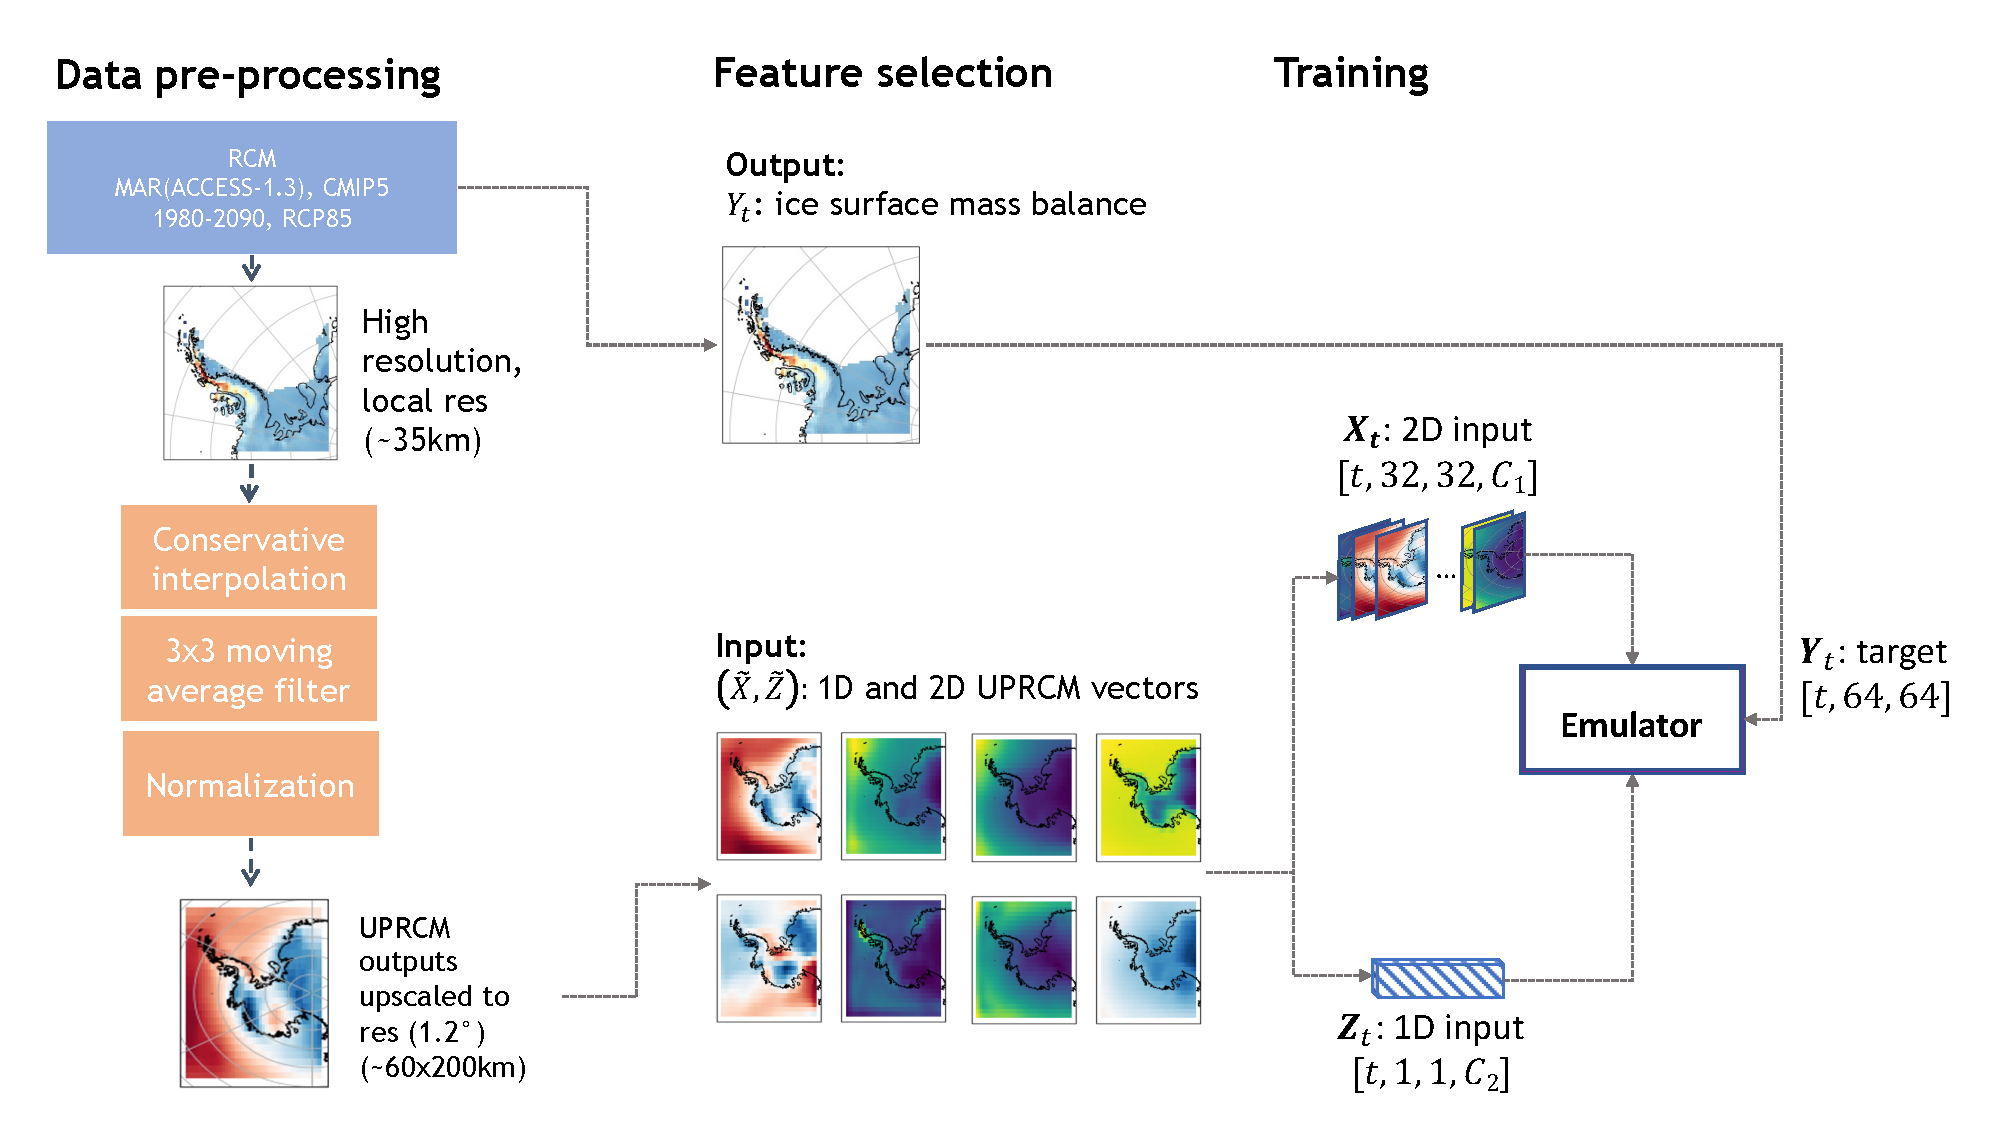
\includegraphics[width=\columnwidth]{images/data-flow.pdf}
  \caption []{\small RCM data flow to create UPRCM data.}
  \vspace{-3mm}
  \label{fig:training-data-flow}
\end{figure}

\section{Architecture selection}
We measured the impact of adding convolutional block attention mechanisms (CBAM) and depth-wise convolutions (DSC) to the U-Net. We compared the performance of the U-Net with and without CBAM and DSC modules and measured the evaluation metrics from~\autoref{subsec:evaluation-metrics} (\autoref{tab:compare-models}). We calculated the percentage of improvement in metrics when going from the basic RCM-emulator to the U-Net with CBAM and DSC for $\mathrm{\hat{F}_{U}(UPRCM)}$ and $\mathrm{\hat{F}_{G}(GCM)}$. The greatest metric improvement was for the Wasserstein distance, which decreased by 26\% and 28\%. CBAM and DSC had a smaller impact on the rest of the metrics. RMSE decreased by 9\% and 7\%, and NRMSE by 10\% and 7\%. The Pearson correlation coefficient was slightly better for the basic model with a -1\% and -2\%. Regarding computational time, training with CBAM and DSC gave a 3 minutes gain. Although the improvement in predictions was not that impressive when adding CBAM and DSC, we still decided to use them in our architecture because of the impact on the Wasserstein distance and the smaller architecture. 

\newpage
\begin{landscape}
% Please add the following required packages to your document preamble:
% \usepackage{multirow}
\begin{table}[tbp]
    \centering
    \caption{}
    \renewcommand\arraystretch{1.5}
\begin{tabular}{clllllllrrr}
\multicolumn{1}{l}{}         &                             & \multicolumn{3}{c}{Without Attention}                                                                 & \multicolumn{3}{c}{Attention - $\mathrm{\hat{F}_{U}(UPRCM)}$}                                                       & \multicolumn{3}{c}{Attention - $\mathrm{\hat{F}_{G}(GCM)}$}                                                        \\ \hline
\multicolumn{1}{l}{}         & \multicolumn{1}{l|}{LR}     & \multicolumn{1}{c}{0.1}      & \multicolumn{1}{c}{0.01}      & \multicolumn{1}{c|}{0.005}             & \multicolumn{1}{c}{0.1} & \multicolumn{1}{c}{0.01} & \multicolumn{1}{c|}{0.005}             & \multicolumn{1}{c}{0.1}      & \multicolumn{1}{c}{0.01}     & \multicolumn{1}{c}{0.005}    \\ \hline
\multirow{4}{*}{RMSE}        & \multicolumn{1}{l|}{min}    & 0.1711                     & 0.1439                      & \multicolumn{1}{l|}{0.1494}          & 0.1686                & 0.1483                 & \multicolumn{1}{l|}{0.1389}          & 0.1687                     & 0.1432                     & 0.1463                     \\
                             & \multicolumn{1}{l|}{mean}   & 1.2909                     & \textbf{1.1904}             & \multicolumn{1}{l|}{1.2475}          & 1.1919                & 1.0931                 & \multicolumn{1}{l|}{\textbf{1.0734}} & 1.1982                     & \textbf{1.0978}            & 1.1054                     \\
                             & \multicolumn{1}{l|}{median} & 0.8682                     & 0.7428                      & \multicolumn{1}{l|}{0.7454}          & 0.7629                & 0.6981                 & \multicolumn{1}{l|}{0.6904}          & 0.7156                     & 0.6967                     & 0.7081                     \\
                             & \multicolumn{1}{l|}{max}    & 7.0078                     & 6.1929                     & \multicolumn{1}{l|}{8.5094}          & 7.1384                & 5.9493                 & \multicolumn{1}{l|}{6.2150}          & 8.7846                     & 6.5332                     & 7.3255                     \\ \hline
\multirow{4}{*}{NRMSE}       & \multicolumn{1}{l|}{min}    & 0.0023                     & 0.0019                      & \multicolumn{1}{l|}{0.0019}          & 0.0023                & 0.0020                 & \multicolumn{1}{l|}{0.0019}          & 0.0023                     & 0.0019                     & 0.0020                     \\
                             & \multicolumn{1}{l|}{mean}   & 0.0172                     & \textbf{0.0159}             & \multicolumn{1}{l|}{0.0167}          & 0.0159                & 0.0146                 & \multicolumn{1}{l|}{\textbf{0.0143}} & 0.0160                     & \textbf{0.0147}            & 0.0148                     \\
                             & \multicolumn{1}{l|}{median} & 0.0116                     & 0.0099                      & \multicolumn{1}{l|}{0.0099}          & 0.0102                & 0.00932                 & \multicolumn{1}{l|}{0.0092}          & 0.0096                     & 0.0093                     & 0.0095                     \\
                             & \multicolumn{1}{l|}{max}    & 0.0936                     & 0.0827                      & \multicolumn{1}{l|}{0.1136}          & 0.0953                & 0.0794                 & \multicolumn{1}{l|}{0.0830}          & 0.1173                     & 0.0872                     & 0.0978                     \\ \hline
\multirow{4}{*}{Wasserstein} & \multicolumn{1}{l|}{min}    & 0.0782                     & 0.0262                      & \multicolumn{1}{l|}{0.0283}          & 0.0508                & 0.0379                 & \multicolumn{1}{l|}{0.0269}          & 0.0417 & 0.0386 & 0.0334 \\
                             & \multicolumn{1}{l|}{mean}   & 0.7013                     & 0.5653                      & \multicolumn{1}{l|}{\textbf{0.4979}} & 0.5722                & 0.3742                 & \multicolumn{1}{l|}{\textbf{0.3663}} & 0.4897                     & \textbf{0.3575}            & 0.3585                     \\
                             & \multicolumn{1}{l|}{median} & 0.5559                     & 0.3284                      & \multicolumn{1}{l|}{0.2572}          & 0.4127                & 0.2595                 & \multicolumn{1}{l|}{0.2680}          & 0.3322                     & 0.2554                     & 0.2392                     \\
                             & \multicolumn{1}{l|}{max}    & 3.4777                     & 3.0174                      & \multicolumn{1}{l|}{4.5005}          & 3.1355                & 2.3569                 & \multicolumn{1}{l|}{2.5277}          & 5.0815                     & 2.6017                     & 2.2302                     \\ \hline
\multirow{4}{*}{Pearson}     & \multicolumn{1}{l|}{min}    & \multicolumn{1}{l}{0.0421} & \multicolumn{1}{l}{-0.0038} & \multicolumn{1}{l|}{0.0858}          & -0.1127               & 0.0720                 & \multicolumn{1}{l|}{0.0725}          & 0.0009                     & 0.0493                     & 0.0469                     \\
                             & \multicolumn{1}{l|}{mean}   & 0.5616 & \textbf{0.5988}             & \multicolumn{1}{l|}{0.5749}          & 0.5263                & 0.5818                 & \multicolumn{1}{l|}{\textbf{0.5893}} & 0.5789                     & 0.5824                     & \textbf{0.5879}            \\
                             & \multicolumn{1}{l|}{median} & 0.5651                     & 0.5839                      & \multicolumn{1}{l|}{0.5685}          & 0.536743                & 0.563422                 & \multicolumn{1}{l|}{0.5733}          & 0.5715                     & 0.5625                     & 0.5689                     \\
                             & \multicolumn{1}{l|}{max}    & 0.9641                     & 0.9662                      & \multicolumn{1}{l|}{0.9499}          & 0.9742                & 0.9766                 & \multicolumn{1}{l|}{0.9715}          & 0.9623                     & 0.9601                     & 0.9794                    
\end{tabular} \subcaption*{\small Table~\ref{tab:compare-models}.  Comparison of three models according to four evaluation metrics calculated between final SMB predictions and RCM-truth. From top to bottom: RMSE, normalized RMSE, Wasserstein distance, and Pearson correlation coefficient. From left to right: U-Net without attention mechanisms and DSC, U-Net trained on UPRCM and evaluated on UPRCM, and U-Net trained on GCM and evaluated on GCM. All models were trained for 50 epochs with early stopping, NRSME loss, and three initial learning rates: 0.1, 0.01, and 0.005. }
            \label{tab:compare-models}
\end{table}
\end{landscape}



\end{document}